\documentclass[a4paper,12pt,twoside,openright,titlepage]{book}

%Additional packages
\usepackage[ascii]{inputenc}
\usepackage[T1]{fontenc}
\usepackage[dutch,english]{babel}
\usepackage{syntonly}
\usepackage[official]{eurosym}
%\usepackage[graphicx]
\usepackage{graphicx}
\graphicspath{ {./images/} }
\usepackage{float}
\usepackage{xurl}
\usepackage{hyperref}
\hypersetup{colorlinks=true, linkcolor=blue, citecolor=blue, filecolor=blue, urlcolor=blue, pdftitle=, pdfauthor=, pdfsubject=, pdfkeywords=}
\usepackage{tabularx}
\usepackage{scrextend}
\addtokomafont{labelinglabel}{\sffamily}
\usepackage{listings}
\usepackage{adjustbox}

%define inch
\usepackage{mathpazo,amsmath}
\def\inch#1{#1''}

% Turn on indexing
\usepackage{imakeidx}
\makeindex[intoc]

% Define colors
\usepackage{color}
\definecolor{ashgrey}{rgb}{0.7, 0.75, 0.71}

% Listing style
\lstset{
  backgroundcolor=\color{ashgrey},   % choose the background color; you must add \usepackage{color} or \usepackage{xcolor}; should come as last argument
  basicstyle=\footnotesize,        % the size of the fonts that are used for the code
  breakatwhitespace=false,         % sets if automatic breaks should only happen at whitespace
  breaklines=true,                 % sets automatic line breaking
  extendedchars=true,              % lets you use non-ASCII characters; for 8-bits encodings only, does not work with UTF-8
  frame=single,	                   % adds a frame around the code
  keepspaces=true,                 % keeps spaces in text, useful for keeping indentation of code (possibly needs columns=flexible)
  rulecolor=\color{black},         % if not set, the frame-color may be changed on line-breaks within not-black text (e.g. comments (green here))
  showspaces=false,                % show spaces everywhere adding particular underscores; it overrides 'showstringspaces'
}

% Uncomment for production
% \syntaxonly

% Style
\pagestyle{headings}

%%%%%%%%%%%%%%%%%%
% Begin document %
%%%%%%%%%%%%%%%%%%

% Define document
\author{D. Leeuw}
\title{Virtualisatie en The Cloud}
\date{\today\\v.0.7.0}

\begin{document}
\selectlanguage{dutch}

\maketitle

\copyright\ 2021 Dennis Leeuw\\

\begin{figure}[H]

\includegraphics[width=0.3\textwidth]{CC-BY-SA-NC.png}
\end{figure}

\bigskip

Dit werk is uitgegeven onder de Creative Commons BY-NC-SA Licentie en laat anderen toe het werk te kopi\"eren, distribueren, vertonen, op te voeren, en om afgeleid materiaal te maken, zolang de auteurs en uitgever worden vermeld als maker van het werk, het werk niet commercieel gebruikt wordt en afgeleide werken onder identieke voorwaarden worden verspreid.


%%%%%%%%%%%%%%%%%%%
%%% Introductie %%%
%%%%%%%%%%%%%%%%%%%

\frontmatter
\chapter{Over dit Document}
Dit document behandeld de opslag van data op de verschillende opslagsystemen voor het middelbaar beroepsonderwijs in Nederland.

\section*{Versienummering}
Het versienummer van elk document bestaat uit drie nummers gescheiden door een punt. Het eerste nummer is het major-versie nummer, het tweede nummer het minor-versienummer en de laatste is de nummering voor bug-fixes.\par
Om met de laatste te beginnen als er in het document slechts verbeteringen zijn aangebracht die te maken hebben met type-fouten, websites die niet meer beschikbaar zijn, of kleine foutjes in de opdrachten dan zal dit nummer opgehoogd worden. Als docent of student hoef je je boek niet te vervangen. Het is wel handig om de wijzigingen bij te houden.\par
Als er flink is geschreven aan het document dan zal het minor-nummer opgehoogd worden, dit betekent dat er bijvoorbeeld plaatjes zijn vervangen of geplaatst/weggehaald, maar ook dat paragrafen zijn herschreven, verwijderd of toegevoegd, zonder dat de daadwerkelijk context is veranderd. Een nieuw cohort wordt aangeraden om met deze nieuwe versie te beginnen, bestaande cohorten kunnen doorwerken met het boek dat ze al hebben.\par
Als het major-nummer wijzigt dan betekent dat dat de inhoud van het boek substantieel is gewijzigd om bijvoorbeeld te voldoen aan een nieuw kwalificatiedossier voor het onderwijs. Een nieuw major-nummer betekent bijna altijd voor het onderwijs dat men in het nieuwe schooljaar met deze nieuwe versie aan de slag zou moeten gaan. Voorgaande versies van het document zullen nog tot het einde een schooljaar onderhouden worden, maar daarna niet meer.

\section*{Document ontwikkeling}
Het doel is door middel van open documentatie een document aan te bieden aan zowel studenten als docenten, zonder dat hier hoge kosten aan verbonden zijn en met de gedachte dat we samen meer weten dan alleen. Door samen te werken kunnen we meer bereiken.\par
Bijdragen aan dit document worden dan ook met alle liefde ontvangen. Let u er wel op dat materiaal dat u bijdraagt onder de CC BY-NC-SA licentie vrijgegeven mag worden, dus alleen origineel materiaal of materiaal dat al vrijgegeven is onder deze licentie.\par
De eerste versie is geschreven voor het ROC Horizon College.

\begin{flushleft}
\begin{table}[h!]
\centering
\begin{tabularx}{\textwidth}{ |c|c|c|X| }
\hline
	Versienummer &
	Auteurs &
	Verspreiding &
	Wijzigingen\\
\hline
	0.1.0 &
	Dennis Leeuw &
	Initieel document\\
\hline
\hline
\end{tabularx}
\caption{Document wijzigingen}
\label{table:1}
\end{table}
\end{flushleft}



%%%%%%%%%%%%%%%%%
%%% De inhoud %%%
%%%%%%%%%%%%%%%%%
\tableofcontents

\mainmatter
\chapter{Simulatie, Emulatie en Virtualisatie}\index{Simulatie}\index{Emulatie}\index{Virtualisatie}
Simulatie, emulatie, imitatie en virtualisatie zijn termen die min of meer hetzelfde betekenen in het Nederlands, maar in de IT een verschillende betekenis kunnen hebben. Vergelijk ook met de Engelse woorden simulation, emulation, imitation en virtualization.

Volgens Van Dale is simulatie het verrichten van schijnbare handelingen of ook nabootsen. Nabootsen komen we ook tegen bij imitatie, terwijl bij emulatie iets staat dat niets te maken heeft met wat we in de IT bedoelen. Van Dale geeft er wedijver en naijver, kortom het beter willen doen. Bij virtueel komt komt in Van Dale iets voor waar we echt wat mee kunnen: Slechts schijnbaar bestaand. Zo zie je dat deze termen snel verwarring kunnen opleveren.

Simulation in de IT is wat er bijvoorbeeld in games gebeurd. Een flight simulator doet een vliegtuig na en geeft je het gevoel echt in een vliegtuig te zitten. Veel andere spelletjes zijn ook simulatoren.

Virtualization is het ophakken van bestaande resources in kleine stukjes. Een virtual machine krijgt zo een klein stukje processor gebruik, een klein stukje geheugen, een stukje van een harddisk. 

Emulation doet hetzelfde als virtualization, maar heeft daarnaast de mogelijkheid om een vertaalslag te maken naar ander type hardware of software. Een emulator geeft je bijvoorbeeld de mogelijkheid om een PowerPC chip na te doen op een ix86 processor. De VM denkt dat zijn processor een PowerPC chip is, terwijl er in de onderliggend fysieke hardware bijvoorbeeld een Core i7 van Intel zit.

Dit document behandeld alleen virtualisatie.

\section{Wat is virtualisatie?}
Virtualisatie is dat iets lijkt te zijn wat het niet is. Op Windows-systemen kan bijvoorbeeld een drive gemapd zijn naar de letter G. Dit lijkt een lokale disk, maar in werkelijkheid is het een netwerk-share.

Virtualisatie in de ICT is een heel breed onderwerp dat gaat van opslag tot servers en van desktops tot applicatie containers. Het doel van  dit document is meer helderheid te verschaffen in de terminologie die gebruikt wordt in dit vakgebied en door middel van opdrachten de lezer meer vertrouwd te maken met de technologie.


De eerste computers konden \'e\'en applicatie per keer draaien, na de uitvinding van het besturingssysteem konden er meerdere applicaties tegelijk op een computer draaien, maar was het systeem beperkt tot \'e\'en OS per keer. Met multi-boot werd het mogelijk om soms het ene en soms het andere besturingssysteem op te starten. En tegen woordig kunnen we op \'e\'en computer niet alleen meerdere applicaties draaien maar ook meerder besturingssystemen.

Een goed introductie kan je zien in dit filmpje van IBM:
\url{https://www.youtube.com/watch?v=FZR0rG3HKIk}


\chapter{The Cloud}\index{Cloud}\index{The Cloud}
Tegenwoordig spreken we van cloud oplossingen en van data opslaan in de cloud, maar wat is dat eigenlijk die cloud? De naam cloud komt vermoedelijk van het feit dat in de automatisering als we een netwerk in generieke zin willen weergeven we meestal een wolkje tekenen. Daardoor zijn we diensten die in het netwerk draaien gaan aanduiden als cloud diensten. Het Internet is het belangrijkste netwerk dat we vaak als cloud beschrijven. Cloud diensten draaien dan ook bij een provider ergens op het Internet. Voor de gebruiker is het niet van belang waar die dienst is.

Bij providers kunnen verschillende soorten diensten worden afgenomen: IaaS, PaaS en SaaS.

\section{IaaS}\index{IaaS}\index{Infrastructure as a Service}
Infrastructure as a Service is een dienst die gevirtualiseerde hardware aanbiedt. Je kan dan bijvoorbeeld kiezen voor 2 CPUs, 2 Gig RAM en 300 GB storage met eventueel nog wat eisen en wensen aan het netwerkverkeer dat naar de machine gaat.

Deze dienst is ook bekend onder de term Virtual Private Server.

Meestal kun je een OS kiezen uit een lijst van beschikbare OSen welke dan op je VPS ge\"installeerd wordt. De rest van de configuratie en installatie van de software moet je zelf doen. Je hebt de volledige vrijheid bij de inrichting.

\section{PaaS}\index{PaaS}\index{Platform as a Service}
Platform as a Service is een dienst die je naast een virtuele machine en een besturingssysteem ook de middleware aanbiedt. Je kan bijvoorbeeld een PaaS dienst bestellen met LAMP. Linux, Apache, MySQL en PHP zullen dan al voor je ge\"installeerd zijn en daar hoef je dus niets meer aan te doen. Je bent alleen nog verantwoordelijk voor het installeren van de applicatie (web-applicatie).

PaaS wordt vaak aangeboden onder de naam webhosting.

\section{SaaS}\index{SaaS}\index{Software as a Service}
Software as a Service biedt software aan via het Internet. Je hoeft niets meer te installeren en heb meestal alleen toegang tot de web-interface van de applicatie. Voorbeelden zijn bijvoorbeeld de Google Applicatie Suite en Office 365.


\chapter{Machine Virtualisatie (IaaS)}\index{VM}\index{Virtual Machine}\index{IaaS}\index{Infrastructure as a Service}
Machine virtualisatie zorgt ervoor dat er effici\"enter gebruik wordt gemaakt van computing resources. Moderne computers zijn zo krachtig dat ze met \'e\'en besturingssystemen en een paar applicaties of services vaak meer niets staan te doen dan dat ze werken. Door op deze hardware meerdere besturingssystemen te draaien kunnen de systemen effici\"enter ingezet worden. De grote datacenters hebben dan minder hardware nodig wat bezuinigt op stroomgebruik, warmte ontwikkeling beperkt en kastruimte bespaart.

Om meerdere besturingssystemen op \'e\'en machine te draaien is er iets nodig dat de bestaande hardware ophakt in stukjes zodat deze gezien wordt door de verschillende OSen als 'eigen' hardware. De techniek die daarvoor gebruikt wordt heet een hypervisor.

\section{Hypervisor}\index{Hypervisor}
Een hypervisor is een stuk software die hardware virtualisatie mogelijk maakt. Er bestaan twee type hypervisors; type 1 en type 2.

Hypervisor type 1 is een hypervisor die op bare metal draait. De hypervisor levert zijn eigen besturingssysteem en maakt rechtstreeks gebruik van de beschikbare hardware om deze aan te bieden aan de virtuele machines.

De andere variant is een Hypervisor type 2, deze draait op een bestaand besturingssysteem. Je hypervisor is dus eigenlijk een applicatie op een besturingssysteem en maakt gebruik van het onderliggende besturingssysteem om hardware aan te bieden aan de virtuele machines. Deze laatste techniek is simpeler omdat een type 2 hypervisor gebruik kan maken van de drivers van het OS waarop het draait.

Een hypervisor verdeelt de bestaande hardware op in stukjes en biedt deze aan als een nieuwe machine. De hypervisor doet dus alsof hij allemaal zelfstandige computers aanbiedt, vandaar dat we dat virtuele machines noemen (virtual machines), wat me meestal afkorten als VM. De machine (en het OS) waarop de hypervisor draait wordt de Host genoemd, de virtuele machine die op de hypervisor draait wordt de Guest genoemd.

Het is natuurlijk een hele kunst om alle hardware te ondersteunen en de calls van het Guest OS correct door te zetten naar de hardware. Een andere optie is dat het Guest OS niet een echte netwerkkaart driver gebruikt, maar een pseudo-driver die zich bijvoorbeeld voordoet als een netwerkkaart. We hebben het dan over een vorm van emulatie, binnen de virtualisatie wereld noemen we dat paravirtualisatie. Voor paravirtualisatie is het nodig om het OS aan te passen aan de hypervisor. Dit is bijvoorbeeld noodzakelijk als de hardware onder de hypervisor geen virtualisatie ondersteund.

Bijna alle moderne computers en laptops ondersteunen hardware virtualistie. In de BIOS kan de ondersteuning voor virtualisatie aan of uit gezet worden. De twee grote processor makers van onze wereld, Intel en AMD, hebben de techniek van virtualisatie ondersteuning beide een iets ander naam gegeven. De ondersteuning voor Intel processoren heet VT-x en voor AMD heet het AMD-V.

\subsection{Hypervisor Opdracht}
Herstart je laptop en ga naar de BIOS settings van je computer. Zoek in de BIOS waar de settings staan voor virtualisatie en als deze uit staan ze het dan aan.

\subsection{Disk images}
Als je een operating system installeerd op een hypervisor dan wordt dit ge\"installeerd in een bestand. Een werkelijke harddisk is niet aanwezig in een VM, dus een bestand wordt gebruikt als virtuele harddisk. Deze virtuele harddisk met daarop een ge\"installeerd OS heet een image. Images kunnen op verschillende manieren gemaakt worden.

Als van een harddisk de data bit voor bit gelezen wordt en weggeschreven wordt als bestand dan heet dat bestand een raw-image. Het bestand zal dus net zo groot zijn als de oorspronkelijke grote van de harddisk. Dit neemt veel ruimte in en er kan effici\"enter gebruik gemaakt worden door het bestand bijvoorbeeld te zippen. Naast een image van een harde schijf kan er ook een image gemaakt worden van een CD- of DVD-disk. Deze images worden ISO\index{ISO-image} images genoemd en hebben de \texttt{.iso} extensie.

Verschillende virtualisatie systemen hebben verschillende oplossingen bedacht om minder schijfruimte in te nemen, maar niet de overhead van zippen te hebben. Dit heeft verschillende image formaten opgeleverd.

\section{Hypervisors}
In deze paragraaf behandelen we een aantal van de beschikbare hypervisors op de markt. We geven een overzicht van enkele commeri\"ele versies waarvoor een gratis instap model beschikbaar is en een paar open source producten.

\subsection{VirtualBox}\index{VirtualBox}
VirtualBox, een type 2 hypervisor, is in 2007 uitgebracht door Innotec GmbH die er tevens de broncode bijleverde. Innotec werd in 2008 gekocht door Sun Microsystems die VirtualBox verder ontwikkelde. Sinds 2010 is Sun in handen van Oracle.

VirtualBox disk image: VDI - Virtual Disk Image\index{VDI}\index{Virtual Disk Image}


\subsubsection{VirtualBox: installatie}
\input{src/virtualbox_installatie}
\subsubsection{VirtualBox: een nieuwe VM maken}
Afhankelijk van de versie van VirtualBox kan je via de de knop New of via de menubalk Machine en dan New een nieuwe virtuele machine aanmaken. Het eerste scherm waarmee je geconfronteerd wordt is \ref{VB_New_VM}.
\begin{figure}[H]
	\centering
	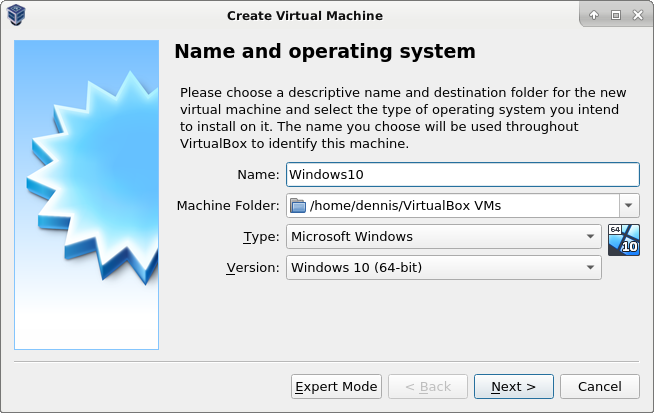
\includegraphics{virtualbox_vm_new.png}
	\caption{VirtualBox: New VM}
	\label{VB_New_VM}
\end{figure}
Op het scherm word je gevraagd om de machine een naam te geven en er wordt gevraagd wat voor virtuele machine je wilt aan maken. Op basis van de keuzes die je maakt bij Type en Version worden er later bepaalde standaard waarden gekozen, die je natuurlijk nog kan wijzigen. Type is het besturingssysteem en Version is de versie van het besturingssysteem dat je later wilt gaan installeren.

Als je je keuzes gemaakt hebt mag je op Next klikken. Daarna zal het scherm verschijnen dat je de mogelijkheid geeft om de hoeveelheid RAM te kiezen die er aan de machine moet worden toegewezen (zie figuur \ref{VB_New_VM_RAM}). Over het algemeen zijn de default waarden goed, mocht je voor een opdracht andere waarden nodig hebben dan kan je ze natuurlijk wijzigen. Het voordeel van virtuele machines is dat je later makkelijk deze settings ook nog kan wijzigen, dus zelfs als je hier geen juiste waarde hebt gekozen, is dat later nog aan te passen. Bij de selectie van de hoeveelheid geheugen is het verstandig om niet meer RAM aan een VM toe te wijzen dan er in je machine zit min de hoeveelheid RAM die nodig is voor de op dat moment gebruikte hoeveelheid RAM. Dit om te voorkomen dat je systeem trager wordt doordat de VM alles gebruikt.

\begin{figure}[H]
	\centering
	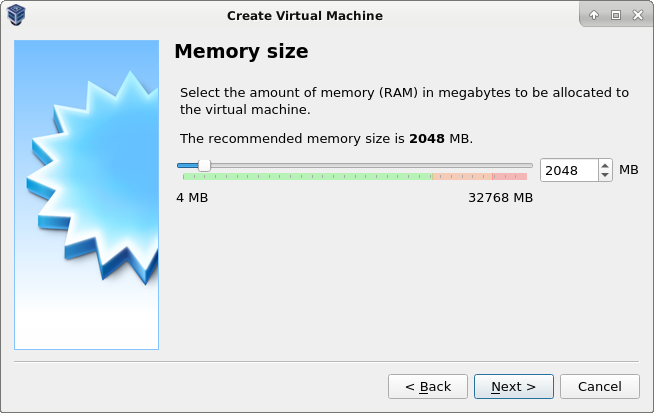
\includegraphics{virtualbox_vm_new_ram.png}
	\caption{VirtualBox: RAM}
	\label{VB_New_VM_RAM}
\end{figure}

Na de keuze voor de hoeveelheid RAM komt de keuze voor de harddisk aanbod. Je kan kiezen uit geen harddisk (figuur \ref{VB_New_VM_HD}), het aanmaken van een nieuwe harddisk of het gebruiken van een bestaand disk-image. Dit is geen echte harddisk. De harddisk van een virtual machine is een bestand dat op de systeemharddisk wordt geschreven, een zogenaamde disk image. Je machine gebruikt dus een bestand als virtuele harddisk. Voor een nieuwe machine maken wij een nieuwe harddisk aan.

\begin{figure}[H]
	\centering
	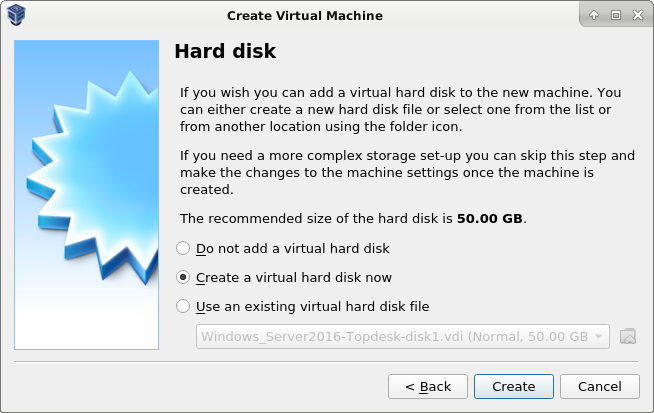
\includegraphics{virtualbox_vm_new_harddisk.png}
	\caption{VirtualBox: Harddisk}
	\label{VB_New_VM_HD}
\end{figure}

Na op Next geklikt te hebben krijg je in \ref{VB_New_VM_HD_Type} de keuze voor het type disk image dat VirtualBox voor je moet aanmaken. Het standaard formaat van VirtualBox is VDI\index{VDI}\index{VirtalBox Disk Image}.

\begin{figure}[H]
	\centering
	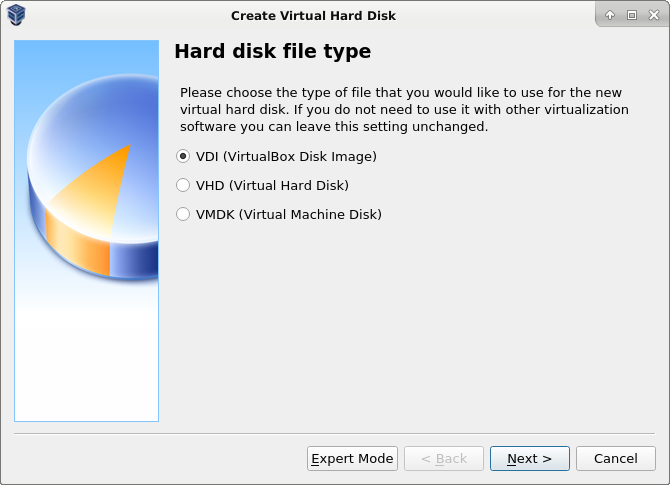
\includegraphics{virtualbox_vm_new_harddisk_type.png}
	\caption{VirtualBox: HD Type}
	\label{VB_New_VM_HD_Type}
\end{figure}

Omdat een VM volledig draait vanuit een bestand op de hardeschijf is er geen noodzaak om meteen alle ruimte in beslag te nemen. De virtuele disk kan dynamisch groeien met het gebruik van de virtuele machine. Een dynamisch groeiende disk is iets trager, maar neemt uiteindelijk minder ruimte in. Deze afweging, tussen ruimte en snelheid, moet je maken bij je keuze in het scherm dat je ziet in \ref{VB_New_VM_HD_Size}.

\begin{figure}[H]
	\centering
	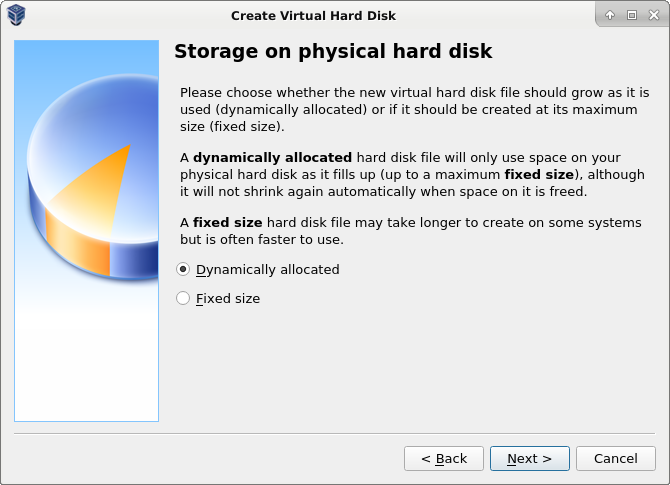
\includegraphics{virtualbox_vm_new_harddisk_size.png}
	\caption{VirtualBox: HD grootte}
	\label{VB_New_VM_HD_Size}
\end{figure}

Tenslotte moet je nog bepalen waar het harddiskbestand en de overige gegevens over je VM worden opgeslagen (zie figuur \ref{VB_New_HD_Location}, ook hier geldt dat de default waarde meestal wel klopt. In dit scherm moet je ook de maximale ruimte voor de virtuele harddisk opgeven. Ook hier is weer een default waarde gegeven. Bepaal zelf of dit het formaat van de harddisk is die je wilt hebben. Afhankelijk van wat je naast het OS nog wil installeren kan je de harddisk groter maken. Let er daarbij vooral op dat je niet meer opgeeft dan je aan vrije diskruimte hebt.

\begin{figure}[H]
	\centering
	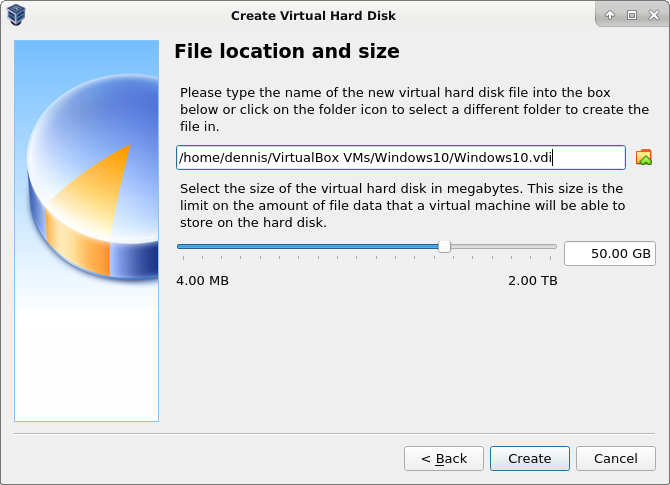
\includegraphics{virtualbox_vm_new_harddisk_location.png}
	\caption{VirtualBox: HD locatie}
	\label{VB_New_VM_HD_Location}
\end{figure}

Klik op Create om de virtuele machine te maken.

\subsubsection{VirtualBox: system settings}
Bij de system settings zitten zitten 3 tabs waaruit je kan kiezen:
\begin{itemize}
	\item Settings die betrekking op het motherboard, o.a. de instelling voor de hoeveelheid RAM van de VM.
	\item Settings die betrekking hebben op de CPU
	\item Settings die betrekking hebben op paravirtualisatie en het nesten van hardware virtualisatie (Acceleration)
\end{itemize}

De belangrijkste instelling bij Motherboard is vermoedelijk de toewijzing van de hoeveelheid RAM aan de VM. Andere opties zijn zaken die je bij een hardware systeem vaak in de BIOS tegen komt zoals de boot order en de tijd zoals deze doorgeven wordt aan het OS. Figuur \ref{VB_settings_system_mb} bevat ook nog andere opties die je kan instellen.
\begin{figure}[H]
	\centering
	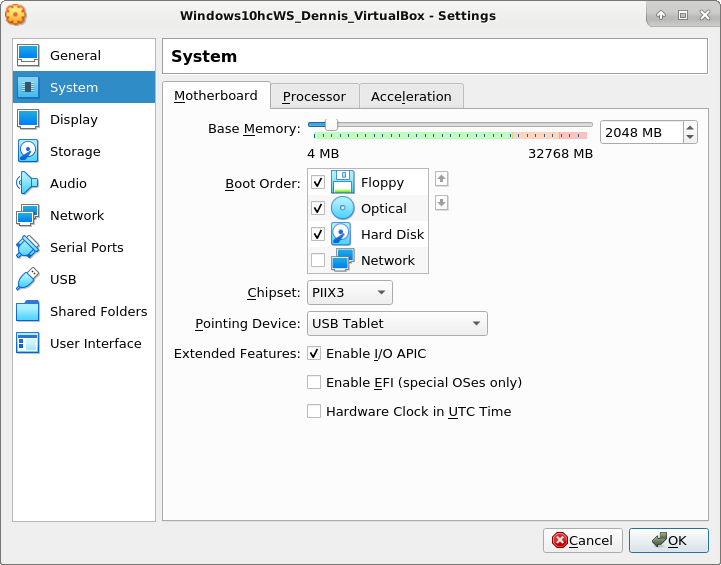
\includegraphics{virtualbox_vm_settings_motherboard.png}
	\caption{VirtualBox New VM}
	\label{VB_settings_system_mb}
\end{figure}

In de tab met Processor (\ref{VB_settings_system_cpu}) kan je aantal cores opgeven dat de VM mag gebruiken en kan je ook opgeven of de hardware virtualisatie doorgeven moet worden aan de VM zodat er nog een hypervisor op de VM ge\"installeerd kan worden.
\begin{figure}[H]
	\centering
	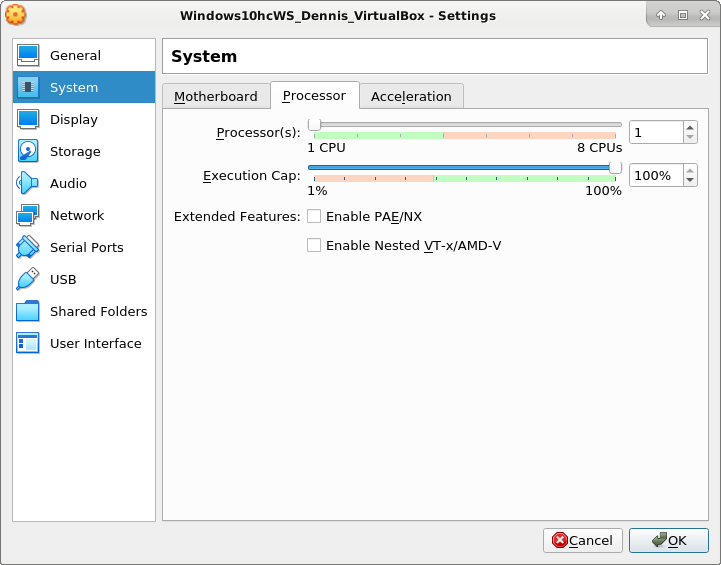
\includegraphics{virtualbox_vm_settings_processor.png}
	\caption{VirtualBox New VM}
	\label{VB_settings_system_cpu}
\end{figure}


\begin{figure}[H]
	\centering
	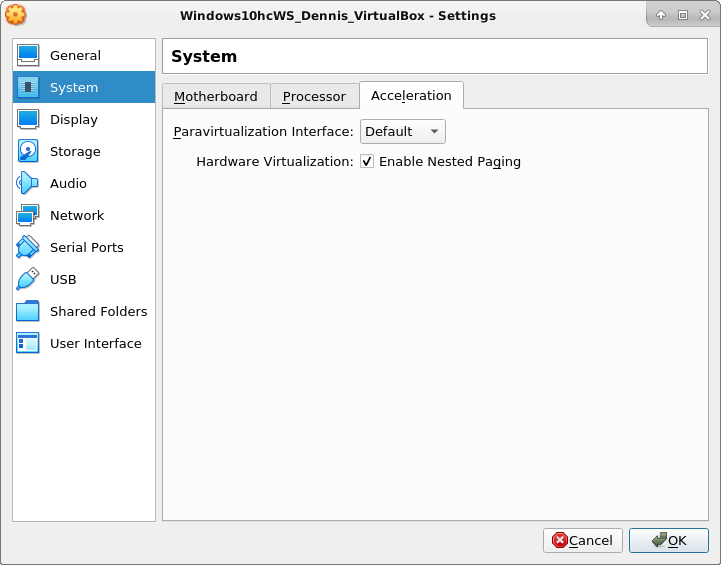
\includegraphics{virtualbox_vm_settings_acceleration.png}
	\caption{VirtualBox New VM}
	\label{VB_New_VM}
\end{figure}


\subsubsection{VirtualBox: OS installatie vanaf een virtuele CD}
Bij Settings vind je ook een item genaamd Storage. In het gepresenteerde overzicht zie je iets dat lijkt op figuur \ref{VB_settings_storage}. Aan de SATA controller hangt je harddisk en een lege CD-ROM speler. Als je de CD-ROM speler aanklikt dan kan je bij het CD-tje aan de rechterkant een CD-image (.iso bestand) toevoegen.
\begin{figure}[H]
	\centering
	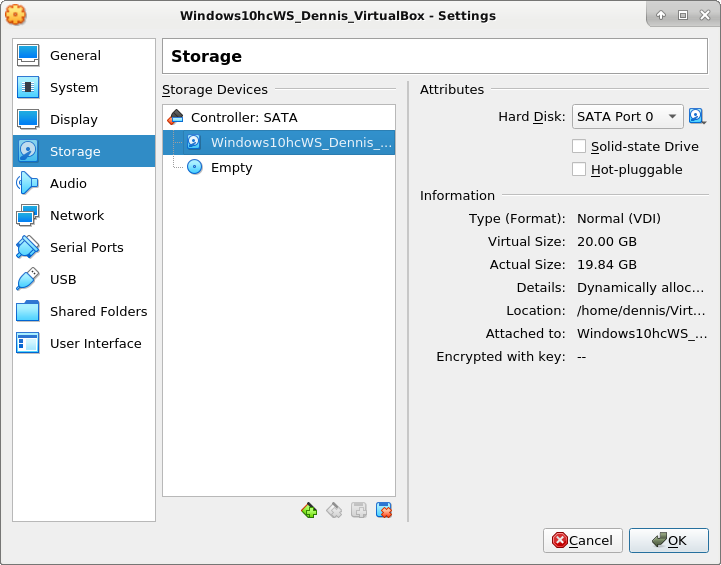
\includegraphics{virtualbox_settings_storage.png}
	\caption{VirtualBox New VM}
	\label{VB_settings_storage}
\end{figure}

Als je het CD-icoontje aanklikt krijg je een menu zoals weergegeven in figuur \ref{VB_settings_storage_cd_add}. Je ziet hier de ISO-images die je eerder gebruikt hebt en je kan ook een nieuwe ISO-image kiezen vanaf de harddisk.
\begin{figure}[H]
	\centering
	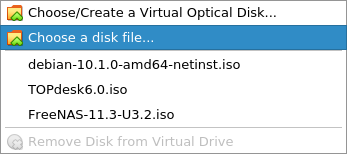
\includegraphics{virtualbox_settings_storage_cd_add.png}
	\caption{VirtualBox New VM}
	\label{VB_settings_storage_cd_add}
\end{figure}

Zodra je je bootable CD-image hebt toegevoegd aan de drive en in de boot order hebt aangegeven dat de CD voor de harddisk geprobeerd wordt, dan zal je systeem opstarten vanaf de (installatie) CD.


\subsection{VMWare}\index{VMWare}
VMWare kwam in 1999 met het product VMWare Player op de markt, vanaf 2015 heet het VMWare Workstation Player. VMWare Workstation Player draait op Windows en Linux en kan x86 systemen virtualiseren. VMWare Workstation Player is een Type 2 hypervisor en draait op een bestaand operating system. Er is ook een VMWare virtualisatie product op de markt voor Mac OS X systemen genaamd VMWare Fusion (beschikbaar vanaf 2006).

In 2001 kwam VMWare ESX op de markt, wat tegenwoordig VMWare ESXi heet, en dat was een type 1 hypervisor met zijn eigen besturingssysteem.

VMDK - Virtual Machine DisK : Since versie 5.0 (2011) is VMDK een open format.

\subsubsection{VMWare: installatie}
Zoek op VMWare Workstation Player Free en download de installatie executable.

\begin{figure}[H]
	\centering
	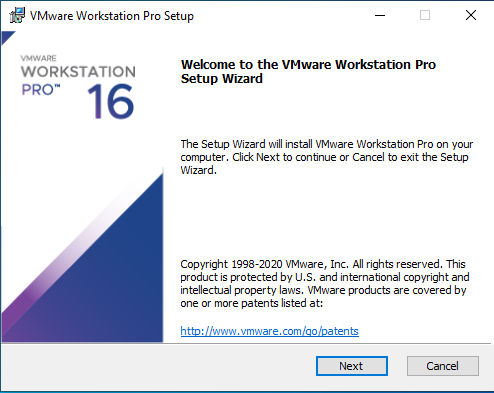
\includegraphics{vmware_ws_install.png}
	\caption{VMWare Workstation Player installatie}
	\label{VW_ws_install}
\end{figure}

\begin{figure}[H]
	\centering
	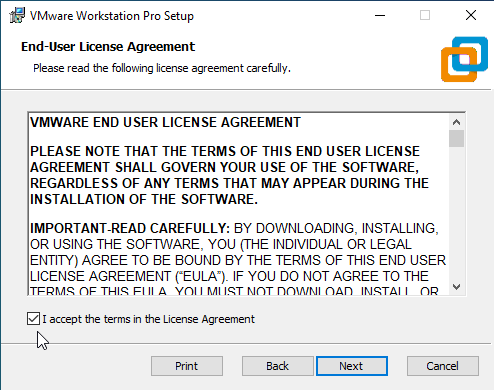
\includegraphics{vmware_ws_lic.png}
	\caption{VMWare Workstation Player installatie}
	\label{VW_ws_install}
\end{figure}

\begin{figure}[H]
	\centering
	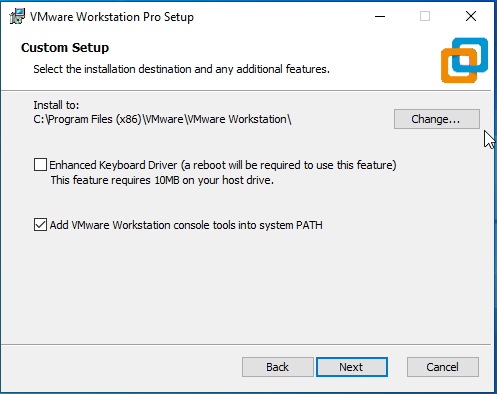
\includegraphics{vmware_ws_setup.png}
	\caption{VMWare Workstation Player installatie}
	\label{VW_ws_install}
\end{figure}

\begin{figure}[H]
	\centering
	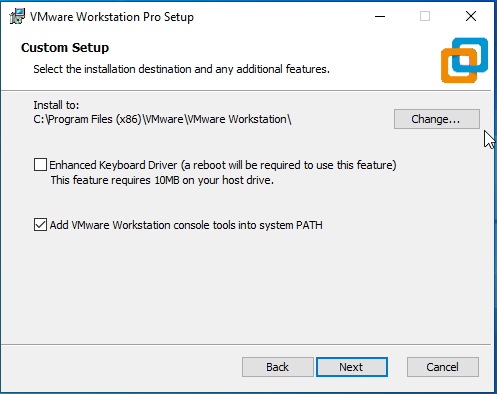
\includegraphics{vmware_ws_setup.png}
	\caption{VMWare Workstation Player installatie}
	\label{VW_ws_install}
\end{figure}

\begin{figure}[H]
	\centering
	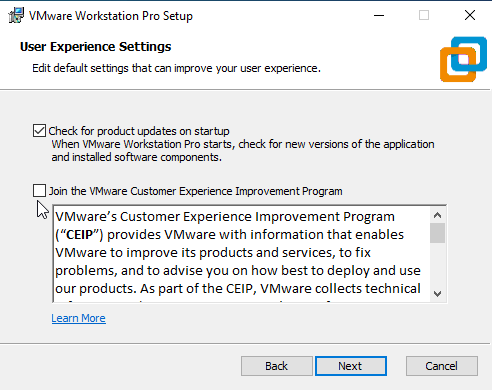
\includegraphics{vmware_ws_exp.png}
	\caption{VMWare Workstation Player installatie}
	\label{VW_ws_install}
\end{figure}

\begin{figure}[H]
	\centering
	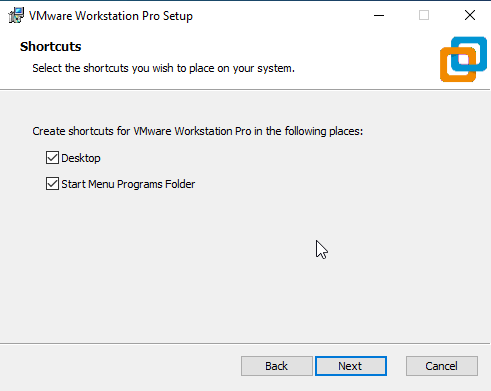
\includegraphics{vmware_ws_shortcuts.png}
	\caption{VMWare Workstation Player installatie}
	\label{VW_ws_install}
\end{figure}

\begin{figure}[H]
	\centering
	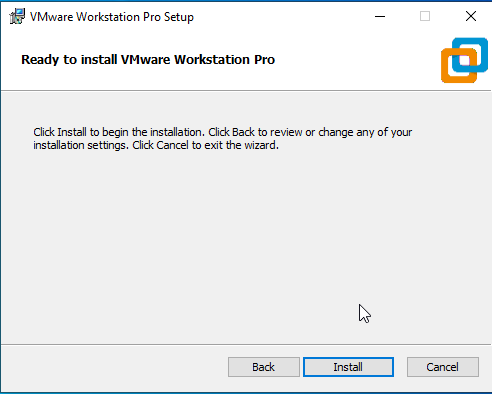
\includegraphics{vmware_ws_install_ready.png}
	\caption{VMWare Workstation Player installatie}
	\label{VW_ws_install}
\end{figure}

Start VMWare Workstation Player en vertel dat we een gratis versie willen gebruiken
\begin{figure}[H]
	\centering
	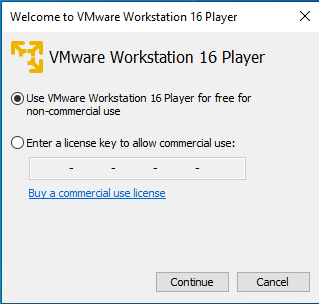
\includegraphics{vmware_ws_run_lic.png}
	\caption{VMWare Workstation Player installatie}
	\label{VW_ws_install}
\end{figure}

\begin{figure}[H]
	\centering
	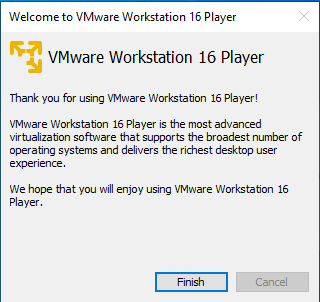
\includegraphics{vmware_ws_run_finish.png}
	\caption{VMWare Workstation Player installatie}
	\label{VW_ws_install}
\end{figure}



\subsubsection{VMWare: een nieuwe VM maken}
Maak een nieuwe virtual machine:

\begin{figure}[H]
	\centering
	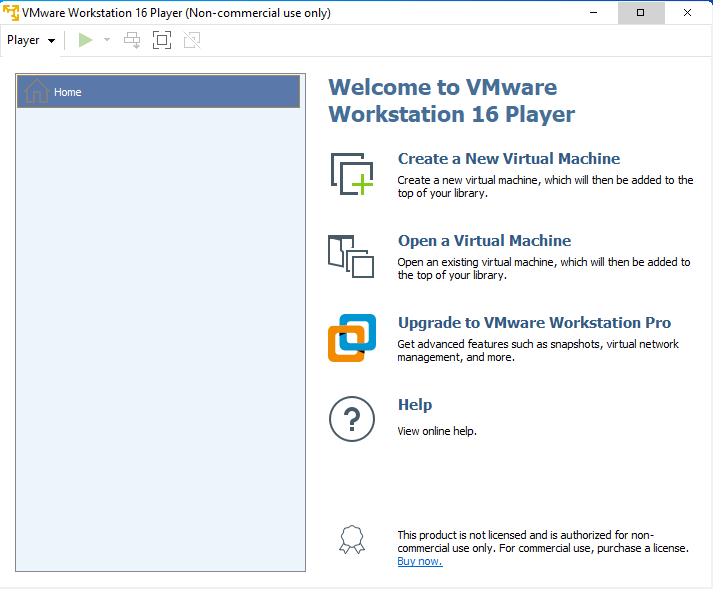
\includegraphics[width=\linewidth]{vmware_ws_vm_new_add.png}
	\caption{VMWare Workstation Player installatie}
	\label{VW_ws_install}
\end{figure}

\begin{figure}[H]
	\centering
	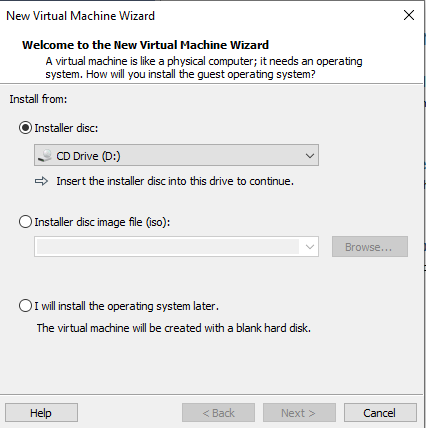
\includegraphics{vmware_ws_vm_new_os.png}
	\caption{VMWare Workstation Player installatie}
	\label{VW_ws_install}
\end{figure}

\begin{figure}[H]
	\centering
	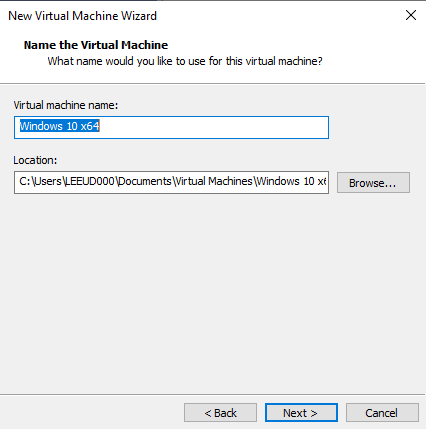
\includegraphics{vmware_ws_vm_new_add_name.png}
	\caption{VMWare Workstation Player installatie}
	\label{VW_ws_install}
\end{figure}

\begin{figure}[h]
	\centering
	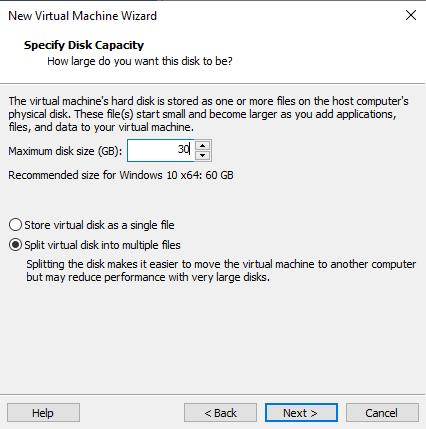
\includegraphics{vmware_ws_vm_new_add_hd.png}
	\caption{vmware workstation player installatie}
	\label{vw_ws_install}
\end{figure}

\begin{figure}[H]
	\centering
	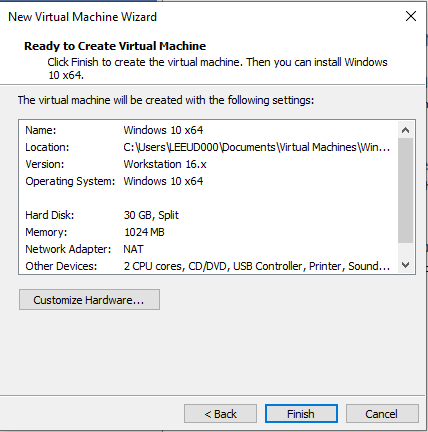
\includegraphics{vmware_ws_vm_new_finish.png}
	\caption{VMWare Workstation Player installatie}
	\label{VW_ws_install}
\end{figure}

\subsection{Xen}\index{Xen}
Op de University of Cambridge begon men met een onderzoeksproject naar een type 1 hypervisor. Het project heette Xen en in 2003 kwam de eerste publieke versie op de markt. Een bedrijf werd opgericht XenSource Inc. die de open source versie beheerde en tevens een commercieel product op de markt bracht. Dit bedrijf werd in 2007 gekocht door Citrix. De open source versie werd ondergebracht bij xen.org. In 2013 kwam de open source Xen ontwikkeling onder de paraplu van de Linux Foundation en ging verder als het Xen Project (xenproject.org).

Citrix ontwikkelde, naast Citrix Xen Server, onder de Xen naam nog enkele andere productie die niets met de Xen hypervisor te maken hebben zoals XenApp en XenDesktop.

Ook andere leveranciers leveren de Xen Hypervisor als een commerieel product, bekende producten zijn:
\begin{itemize}
\item Huawei FusionSphere
\item Oracle VM Server for x86
\item Thinsy Corporation
\item Crucible (hypervisor) by Star Lab Corp
\end{itemize} 


\subsection{KVM}\index{KVM}
KVM is de Linux hypervisor. Het is een kernel module die ook beschikbaar is voor FreeBSD. Het is niet helemaal duidelijk of we KVM nu een type 1 of type 2 hypervisor moeten noemen. De kernel module zorgt ervoor dat de de hypervisor bij de hardware kan, maar de VMs draaien naast de gewone applicaties. Dus het is een soort hybride vorm tussen type 1 en 2 in.

KVM is gestart in 2006 door Avi Kivity en zit sinds 2007 in de mainstream kernel. Het KVM project is gekocht in 2008 door Red Hat en Red Hat is tegenwoordig van IBM.


\subsection{Hyper-V}\index{Hyper-V}
Windows Server 2008 kwam met virtualisatie software genaamd Hyper-V. Hyper-V is een type 1 hypervisor die het bestaande OS tot de eerste VM maakt. Sinds 2012 (Windows 8) is Hyper-V ook beschikbaar voor het Windows desktop besturingssysteem.



\subsubsection{Hyper-V: installatie}
De installatie van Hyper-V op Windows 10 kan met een enkel commando in PowerShell zie \ref{HV_install}.
\begin{figure}[h!]
	\centering
	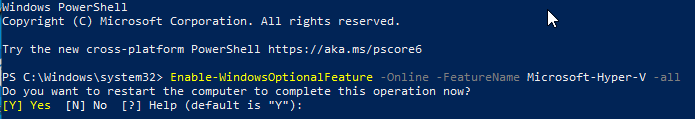
\includegraphics{hyperv_enable_powershell.png}
	\caption{Hyper-V installatie}
	\label{HV_install}
\end{figure}


\subsubsection{Hyper-V: een nieuwe VM maken}
Start de Hyper-V manager als Administrator zodat je voldoende rechten hebt om VMs aan te maken (zie \ref{HV_man_start}
\begin{figure}[H]
	\centering
	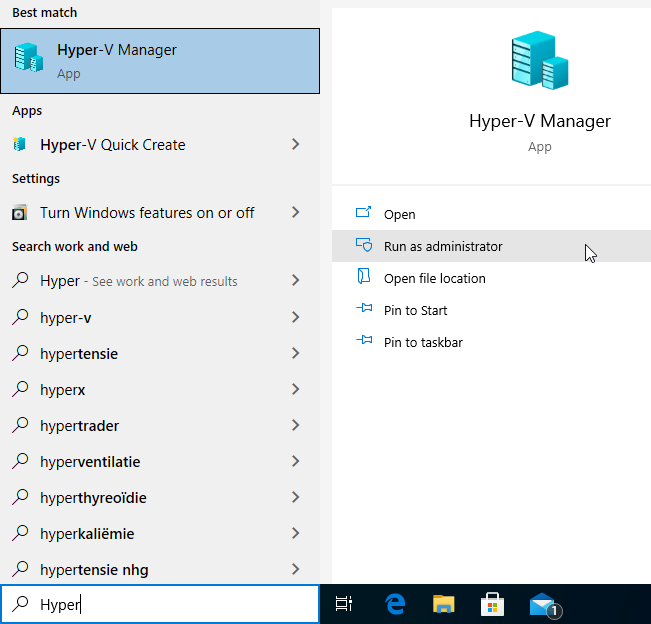
\includegraphics{hyperv_manager_start.png}
	\caption{Hyper-V Manager opstarten}
	\label{HV_man_start}
\end{figure}

Selecteer de server waaraan de manager moet connecten. In de voorbeelden wordt gebruik gemaakt van de Windows 10 desktop machine waarop we Hyper-V ge\"installeerd hebben. De hostname is zichtbaar in de linker kolom (zie \ref{HV_man_server}
\begin{figure}[H]
	\centering
	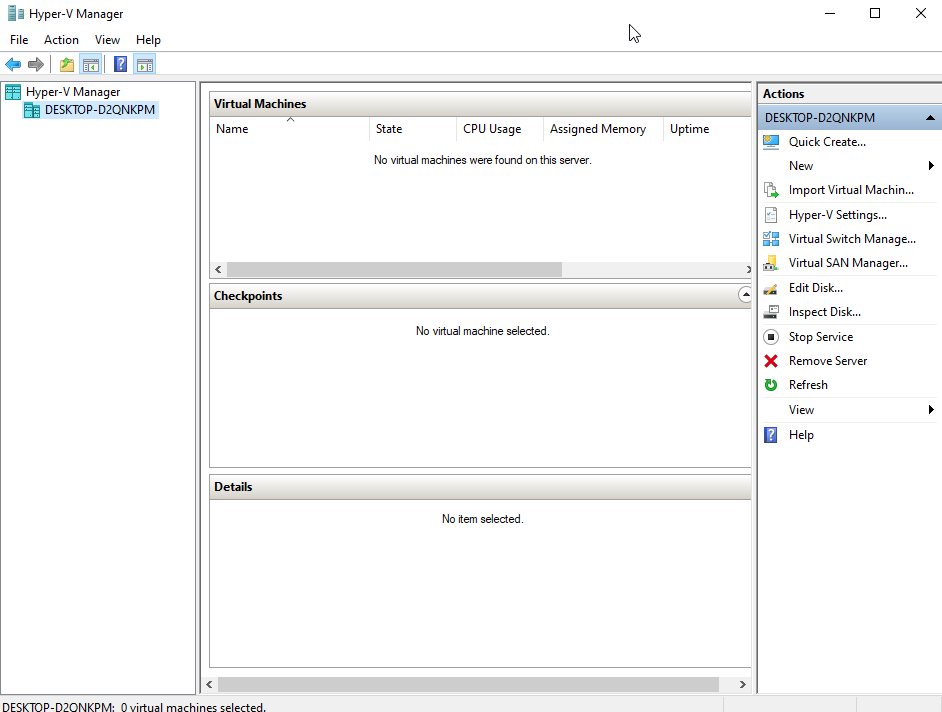
\includegraphics[width=\linewidth]{hyperv_manager_server.png}
	\caption{Hyper-V selecteer de hypervisor die je wil managen}
	\label{HV_man_server}
\end{figure}

Aan de rechterkant selecteer de New (\ref{HV_man_vm_new}) optie en kies Virtual Machine...
\begin{figure}[H]
	\centering
	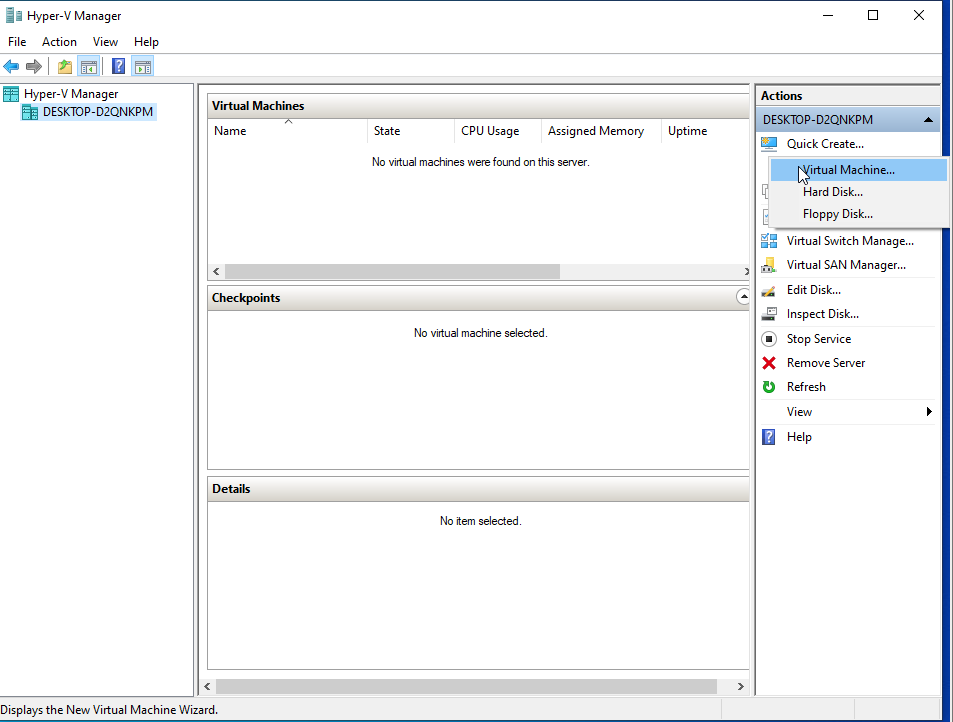
\includegraphics[width=\linewidth]{hyperv_manager_vm_new.png}
	\caption{Hyper-V installatie}
	\label{HV_man_vm_new}
\end{figure}

De eerste pagina is een introductie zoals te zien is in \ref{HV_vmnew_begin}.
\begin{figure}[H]
	\centering
	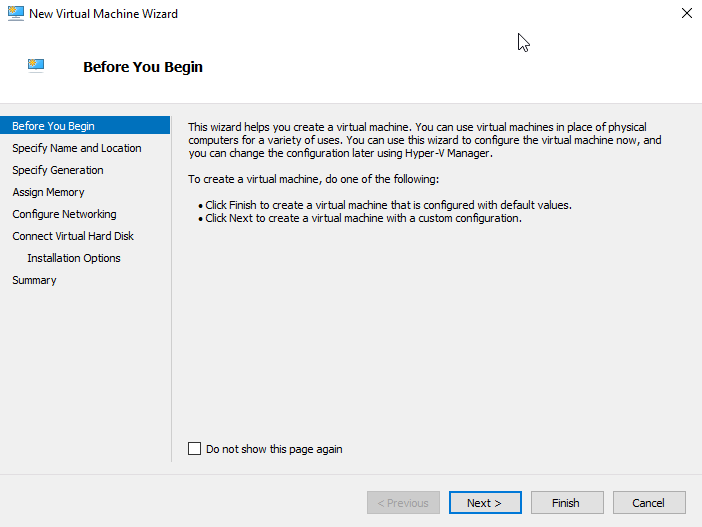
\includegraphics{hyperv_vmnew_begin.png}
	\caption{Hyper-V de begin pagina voor het maken van een nieuwe VM}
	\label{HV_vmnew_begin}
\end{figure}

Na het klikken op Next kom je in het volgende scherm terecht waar we de machine een naam gaan geven (\ref{HV_vmnew_name}
\begin{figure}[H]
	\centering
	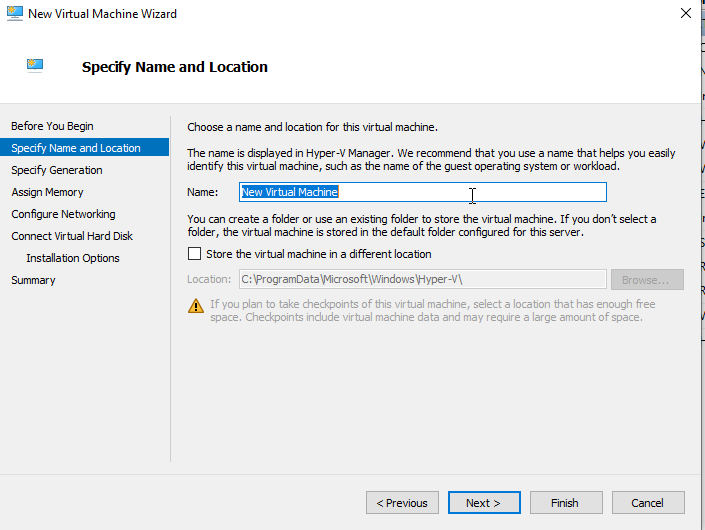
\includegraphics{hyperv_vmnew_name.png}
	\caption{Hyper-V geef de VM een naam}
	\label{HV_vmnew_name}
\end{figure}

Selecteer de generatie. De beschrijving geeft al aan dat Generatie 1 32- en 64-bits systemen kan doen en Generatie 2 alleen 64-bits systemen (\ref{HV_vmnew_gen}
\begin{figure}[H]
	\centering
	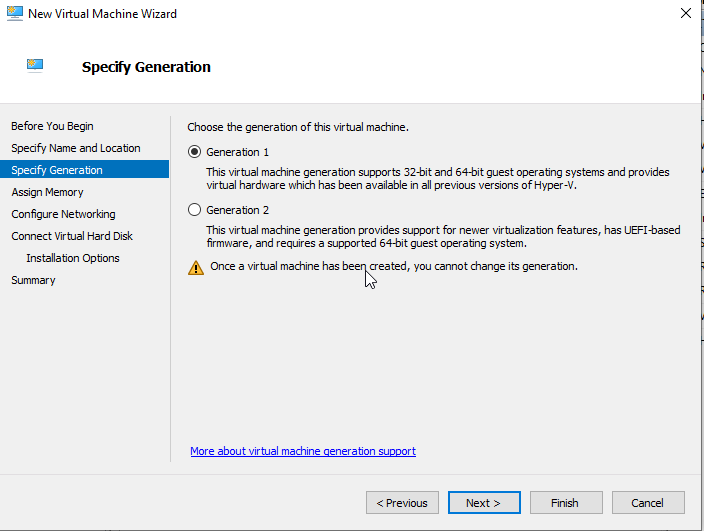
\includegraphics{hyperv_vmnew_gen.png}
	\caption{Hyper-V selecteer de VM generatie}
	\label{HV_vmnew_gen}
\end{figure}

Daarna moeten we bepalen hoeveel RAM deze virtuele machine mag gebruiken \ref{HV_vmnew_ram}
\begin{figure}[H]
	\centering
	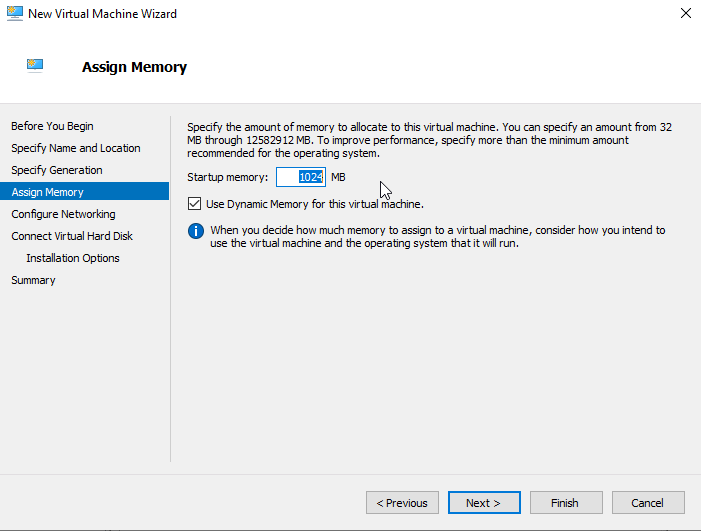
\includegraphics{hyperv_vmnew_ram.png}
	\caption{Hyper-V kies de hoeveelheid RAM voor je VM}
	\label{HV_vmnew_ram}
\end{figure}

Voor de netwerk configuratie is er een nieuwe installatie van Hyper-V alleen het default netwerk aanwezig (\ref{HV_vmnew_net}. Het aanmaken van nieuwe netwerken wordt in een volgende paragraaf besproken.
\begin{figure}[H]
	\centering
	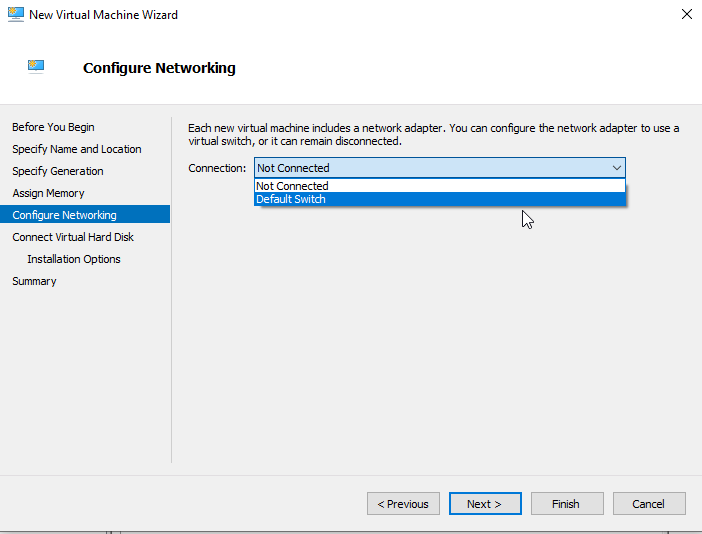
\includegraphics{hyperv_vmnew_net.png}
	\caption{Hyper-V netwerk configuratie}
	\label{HV_vmnew_net}
\end{figure}

We moeten in figuur \ref{HV_vmnew_hd} bepalen hoe groot de harddisk moet worden.
\begin{figure}[H]
	\centering
	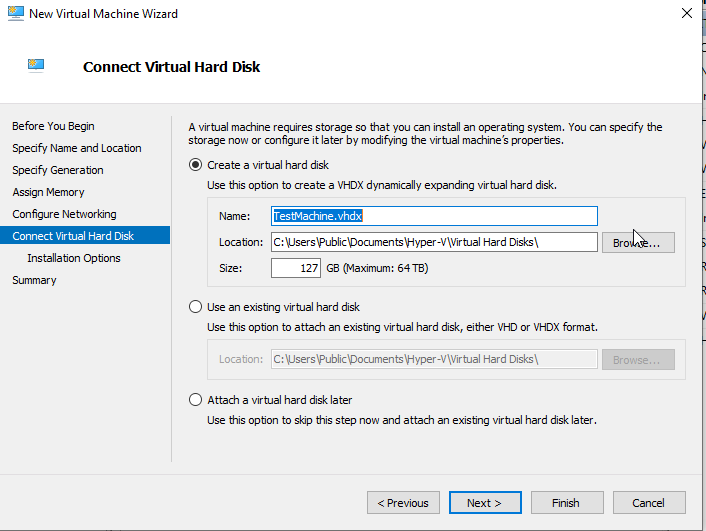
\includegraphics{hyperv_vmnew_hd.png}
	\caption{Hyper-V Harddisk configuratie}
	\label{HV_vmnew_hd}
\end{figure}

Bij Hyper-V krijgen we bij het aanmaken van een VM de vraag of we een OS willen installeren en zo ja waar deze vandaan moet komen. We kunnen selecteren om het systeem op te starten vanaf een ISO-image (\ref{HV_vmnew_os}.
\begin{figure}[H]
	\centering
	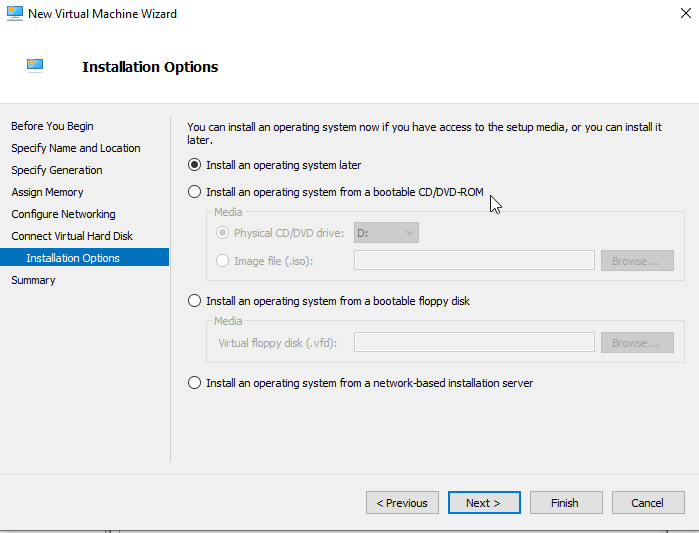
\includegraphics{hyperv_vmnew_osinst.png}
	\caption{Hyper-V Bepaal hoe je een OS op de VM gaat installeren}
	\label{HV_vmnew_os}
\end{figure}

Tenslotte krijg je een overzicht met de gekozen opties en kan je via Finish de creatie van de VM voltooien (\ref{HV_vmnew_finish}
\begin{figure}[H]
	\centering
	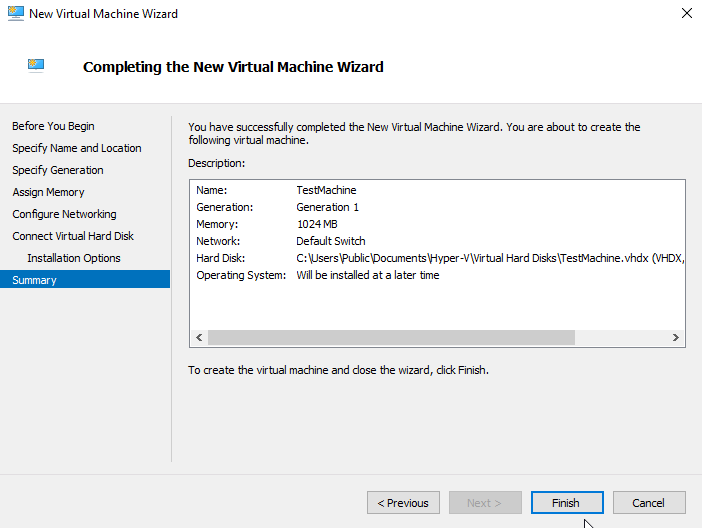
\includegraphics{hyperv_vmnew_summ.png}
	\caption{Hyper-V het daadwerkelijk aanmaken van de VM}
	\label{HV_vmnew_finish}
\end{figure}


\subsection{Parallels}\index{Parallels}
Parallels biedt een gratis proefversie van hun product Parallels Desktop product die het mogelijk maakt om Windows op een Mac OS X machine te draaien. Er is ook een versie voor Chrome. Sinds 2018 is Parallels onderdeel van Corel Corporation.

Parallels draait op Mac OS X en kan als guest OS Windows, Linux en Mac OS X draaien.

HDD - Parallels disk image format

\subsection{Hypervisors opdracht}
Converteer een VDI disk image van VirtualBox naar het VMDK formaat (tip: gebruik qemu-img).

\section{Server virtualisatie}\index{Server virtualisatie}
In de datacentra van providers of bedrijven draaien er servers en desktops als virtuele machines. De eisen voor virtuele servers en desktops verschillen van elkaar. In deze paragraaf zullen we de server virtualisatie behandelen. We hebben het dan voornamelijk over servers die draaien op 19\inch machines en blades. De gevirtualiseerde machines zijn vaak servers die bijvoorbeeld dienen als database- of webserver. Een andere veel gebruikte toepassing is als rekennodes in rekenclusters.

Bij de eerste webservers draaiden bijvoorbeeld Apache en MySQL op \'e\'en en dezelfde server. Dit was hardware en de performance van de website was afhankelijk van de kracht van de fysieke machine. Al snel werden websites groter dan \'e\'en fysieke machine aankon. De functionaliteit werd gesplitst en de database server kreeg zijn eigen machine. Natuurlijk werd dit uiteindelijk ook te klein en werden er database clusters neergezet en kwamen er vele webservers die dezelfde website aanboden. Via loadbalancing werd de totale vraag naar een bepaalde website verdeeld over de verschillende servers. Zie voor een overzicht figuur \ref{fig:WSDB-network}.

\begin{figure}[H]
\includegraphics[scale=0.75]{loadbalancer_en_DB_cluster.png}
\centering
\caption{Webservers met loadbalancer en DB cluster}
\label{fig:WSDB-network}
\end{figure}

Een loadbalancer\index{loadbalancer} is een apparaat dat aan de Internet kant een vraag voor een dienst of een IP adres aanneemt en deze doorzet naar \'e\'en van de servers die hij aan de interne kant heeft. Door voor elke vraag een andere server te gebruiken worden de aanvragen vanaf het Internet verdeeld over verschillende machines zodat de de load verdeeld wordt. Elke server krijgt dus maar een deel van de aanvragen te verwerken. Het is hierbij van belang de alle servers op dezelfde manier zijn ingericht.

Voor het serverpark met webservers worden vaak virtuele machines gebruikt zodat er op een eenvoudige manier \'e\'en master image gemaakt kan worden die uitgerold wordt over de verschillende virtual machines en er zo gelijke webservers ontstaan. De images van de servers staan veelal op de SAN.

MySQL kan ge\"installeerd worden als stand-alone server of als cluster. In een cluster opzet werken de MySQL servers samen om te zorgen dat de database consistent is zodat een query op elk van de servers hetzelfde antwoord geeft. De database draait in het geheugen en wordt verdeeld over de verschillende harddisks opgeslagen. Het cluster gebruikt dus geen SAN, beter is het om het cluster op te vatten als \'e\'en grote database. De verschillende clusternodes kunnen prima draaien op een hypervisor, of beter op verschillende hypervisors.

\subsection{Rekenclusters}\index{Rekencluster}
Rekenclusters zijn verzamelingen van machines die gebruikt worden om complexe rekentaken uit te voeren. We kunnen rekenclusters onderscheiden in twee smaken, de clusters die voornamelijk rekenen met integers (dus gehele getallen) en de clusters die voornamelijk rekenen met floats (dus getallen met cijfers achter de komma). Voor de eerste rekenclusters volstaan meestal de standaard processoren. De rekenclusters die met floats werken hebben vaak voordeel bij het gebruik van GPU's als rekenunits. De Engelse term voor een rekencluster is High Performance Cluster en de techniek heet dan ook High Performance Computing.

Omdat de wensen per rekenopdracht sterk kunnen verschillen, veel CPU power of just veel geheugen, worden de nodes van een rekencluster vaak gevirtualiseerd aangeboden zodat er snel en effici\"ent geschaald kan worden. De overhead van de hypervisor is minder belangrijk dan de schaalbaarheid van het totale cluster waarbij nodes flexibel toegevoegd of verwijderd kunnen worden aan bepaalde rekentaken.

\subsection{High Availibility}\index{High Availibility}
Met alles en iedereen verbonden aan het Internet is het niet meer te zeggen wie wanneer van een dienst gebruik wil maken. De gebruikers kunnen van overal op de wereld komen en dus moeten diensten 24-uur per dag en 7 dagen in de week beschikbaar zijn. Servers mogen niet meer uitvallen en als ze toch uitvallen mag het de dienstverlening niet verstoren. Deze hoge beschikbaarheid of wel high-availibilty is steeds meer de norm, dan de uitzondering.

In de vorige paragrafen hebben we gezien dat de huidige infrastructuur vraagt om schaalbaarheid (scalability) en continu\"iteit (continuity). Deze worden ingegeven door de business ofwel het gaat om business continuity. Het enkele uren down zijn van het netwerk bij een klein advocaten kantoor kan al schadelijk zijn voor de reputatie of zelfs gevolgen hebben voor cli\"enten als als de stukken niet optijd zijn ingeleverd bij de rechtbank. In een ziekenhuis kan het levens kosten. De afhankelijkheid van IT in onze samenleving is heel groot en elke keer zal er een afweging gemaakt moeten worden tussen de kosten en de wens om altijd online te zijn.

Om de uptime zo hoog mogelijk te maken en daarmee de availablity wordt vaak gebruik gemaakt van het dubbel uitvoeren van componenten. Switches worden dubbel uitgevoerd, netwerkkabels worden redundant aangesloten, systemen worden in clusters gezet en naast voeding uit het stroomnet worden er UPSen en aggregaten neergezet. Alles om er maar voor te zorgen dat de systemen blijven werken. Sommige bedrijven gaan zelfs zo ver dat de datacenters dubbel worden uitgevoerd.

Het niet leveren van een bepaalde dienstverlening levert downtime op. Dit kan worden opgevangen door systemen of onderdelen van systemen dubbel uit te voeren. Zo kan een computer uitgerust zijn met een redundante voeding en/of harddisk. Redundant betekent dat de bijvoorbeeld de voeding niet operationeel is, maar alleen als de primaire voeding ermee stopt neemt de redundante of secundaire voeding het over. Deze techniek staat ook bekend als hot-standby. Alles is aangesloten en zonder enige downtime neemt het redundante apparaat de operationele acties over. De systeembeheerder hoeft achteraf alleen het defecte onderdeel te vervangen, zodat ook een volgende calamiteit opgevangen kan worden. Het vervangen van het defecte onderdeel kan gebeuren terwijl het systeem doordraait en niet uit hoefd. We noemen deze onderdelen dan ook hot-swappable. Alles is erop gebouwd dat het systeem maar niet down hoeft, zodat downtime wordt vermeden.


Om het omvallen van systemen op te vangen wordt er gebruik gemaakt van failover oplossingen. We spreken dan van hot- of cold-standby. Een tweede identieke machine kan klaarhangen in de kast, als de primaire server omvalt kan een systeembeheerder het tweede systeem opstarten en zorgen dat de gebruikers weer kunnen werken. Dit levert natuurlijk downtime op, maar als alles goed voorbereid is kan een server in een halfuur weer operationeel zijn. Dit is de cold-standby oplossing, de tweede server draait niet en is dus koud.
Hot-standby betekent dat de failover-server al draaiend op het netwerk aanwezig is. Op het moment dat de primaire server omvalt neemt de tweede server automatisch zijn functies over. De techniek hierachter is meestal het delen van een IP-adres tussen het primaire en het failover systeem. Beide systemen krijgen op hun netwerk interface \'e\'en IP adres toewijzen dat bij de machine hoort en er is \'e\'en IP adres dat ze delen, het zogenaamde virtuele IP adres. Dit virtuele IP adres wordt gebruikt door de gebruikers om een dienst te benaderen. Wie het virtuele IP adres op zijn netwerkkaart heeft staan handeld dus de dienst af. Normaal gesproken zal dat het primaire systeem zijn. Mocht deze echter uitvallen dan neemt het failover systeem het IP adres over op zijn netwerkkaart en krijgt daardoor alle vragen van de gebruikers te verwerken.

\begin{figure}[H]
	\includegraphics[width=\linewidth]{fs_failover.png}
	\caption{File Server Failover}
	\label{FS_failover}
\end{figure}

Twee dingen zijn hierbij van belang, namelijk dat de data op server 1 gelijk is aan die op server 2. In figuur \ref{FS_failover} synchroniseren server 1 en 2 over een (rode) ethernet cross-cable, op deze manier verstoort de syncronisatie niet de bandbreedte naar de gebruikers. Het andere dat van belang is is dat server 2 moet weten wanneer server 1 niet meer bereikbaar is. Dat laatste wordt bereikt met een heartbeat, zeg maar een soort ping waarbij de servers elkaar in de gaten houden. Als server 2 de heartbeat van server 1 niet meer hoort dan neemt het het virtuele IP adres over. De heartbeat kan over een speciale kabel gaan of over de al bestaande netwerken tussen de twee servers.
\index{Failover}
\subsection{Server hardware}\index{Server hardware}
De meeste datacenters zijn uitgerust met 19''-kasten waarin 19''-servers hangen. De 19''-maat staat voor de breedte van de server. De hoogte van een serverkast wordt uitgedrukt in het aantal U. Een normale server, de zogenaamde pizza-doos, is 1U hoog. Harddisks liggen dan plat in de server. Zwaardere servers met meer harddisks hebben de harddisks vaak rechtop op hun zijkant staan die hot-swappable uit de voorkant van de server getrokken kunnen worden. Deze servers zijn 2U hoog.

\begin{figure}[H]
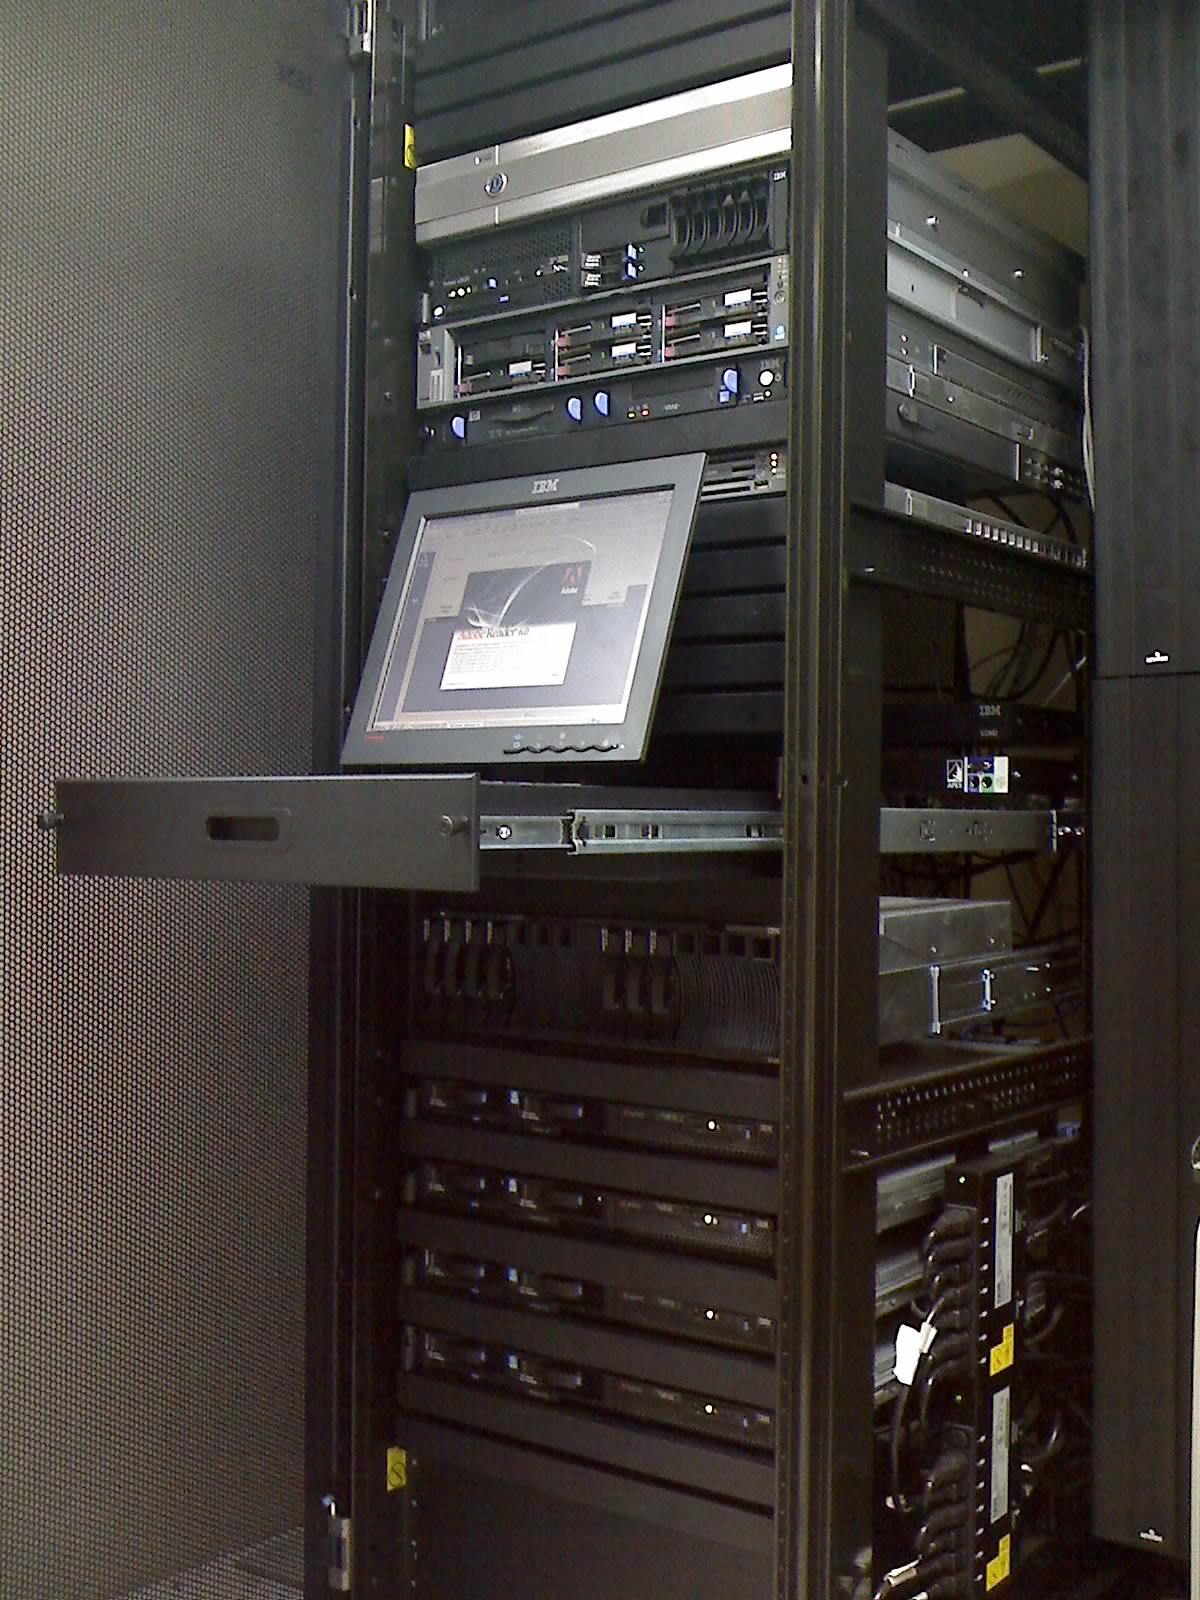
\includegraphics[width=0.75\linewidth]{Wiki_Rack001.jpg}
	\caption{Foto van Jfreyre afkomstig van \url{https://commons.wikimedia.org/wiki/File:Rack001.jpg}}
\centering
\end{figure}

Om hogere dichtheden te bereiken wordt er gebruik gemaakt van blade servers\index{Blade servers}. Bij blade servers zitten er meedere servers (blades) in \'e\'en fysieke behuizing (19''-kast). De servers delen een backplane, de voeding(en) en de behuizing waardoor er effectief meer servers passen op dezelfde oppervlakte. Een nadeel van blades is dat de warmte ontwikkeling ook veel meer geconcentreerd wordt en dat kan leiden tot zogenaamde hotspots, wat slecht is voor de koeling.

\subsection{Server virtualisatie opdrachten}
\begin{enumerate}
\item Zoek op Internet naar een load balancer en schrijf een stuk over welke technieken er gebruikt worden op load balancers. Zijn er ook software oplossingen die je kan inzetten als load balancer?
\item Welke software is er beschikbaar om rekenclusters mee op te zetten?
\item Welke software moet je installeren om een Windows Cluster op te zetten?
\end{enumerate}

\section{The Cloud: Virtual Private Servers}\index{VPS}\index{Virtual Private Server}
Een VPS, Virtual Private Server, is niets anders dan een virtuele server die als dienst aangeboden wordt door een provider (hosting bedrijf). De VPS draait op een server van een aanbieder ergens in zijn of haar datacenter. Een bekende uitspraak in de cloud wereld is daarom niet voor niets "The cloud that is just somebody else's computer".

Het grote voordeel van het gebruik van een VPS is dat al het beheer van het datacentrum, de computers en de netwerken is uitbesteed (ge-outsourced). Hier kan enorm bespaard worden op salarissen, gebouw ruimte en de steeds terug kerende kosten van het aanschaffen van nieuwe systemen. Providers kunnen door hun schaalgrootte goedkoper inkopen en de beheerkosten kunnen ze door relatief laag houden.

Het nadeel is dat de computers niet meer in de eigen datacentra staan en dat de afhankelijkheid van een goed en betrouwbaar Internet toeneemt. Bij een calamiteit met de Internet verbinding kan een heel bedrijf stil komen te liggen.

\section{Virtuele netwerken}
Virtuele machines gebruiken virtuele netwerkkaarten en deze netwerkkaarten zijn gekoppeld aan virtuele netwerkswitches op de host machine. Die virtuele switches of vSwitches, zoals VMWare ze noemt, zijn niet zichtbaar omdat ze uit software zijn gemaakt, maar ze hebben wel effect op het functioneren van de machine. Zo kan een virtuele netwerkkaart direct gekoppeld zijn aan de netwerkkaart van de host en kan de virtuele machine direct met het lokale netwerk van de host praten. Het kan ook zo zijn dat de virtuele netwerkkaart in een virtuele switch zit waar alle andere virtuele machines ook in zitten en een virtuele adapter van het host systeem. Op die manier kan de host met de virtuele machines praten en kunnen de virtuele machines ook onderling met elkaar praten, maar via dit virtuele netwerk kan niemand met de buitenwereld praten.

Er zijn verschillende soorten netwerken die via hypervisors kunnen worden opgebouwd. In de volgende paragrafen zullen we de belangrijkste type netwerk configuraties doornemen.

\subsection{Virtual Network: verbinding met de wereld}
Een netwerk configuratie waarbij de VM alleen naar buiten kan wordt in Hyper-V een External netwerk genoemd en in VirtualBox een NAT netwerk. Dit is bij bijna alle hypervisors het standaard netwerk. De VM is ge\"isoleerd van de host en kan alleen via de netwerkkaart van de host naar het aangesloten netwerk. Een directe verbinding tussen host en VM is niet mogelijk.

Omdat de VM zijn eigen netwerk adressen heeft, al dan niet uitgedeeld door een DHCP-server op de host moeten de interne adressen via NAT (Network Address Translation) vertaald worden naar het externe IP adres van de netwerkkaart van de host om geen conflicten op te leveren op het aangesloten netwerk en om ervoor te zorgen dat antwoorden op connecties naar buiten weer terug worden gerouteerd naar de virtuele machine.

\subsection{Virtual Network: onderlinge verbindingen}
Een virtuele switch waarbij de host en de VMs met elkaar verbonden zijn, maar waarbij er geen verbinding naar buiten is wordt in dit document een management netwerk genoemd, omdat dat is waar het meestal voor gebruikt wordt. Vanaf de host kunnen op deze manier de verschillene VMs gemanaged worden door bijvoorbeeld gebruik te maken van remote desktop applicaties of een andere vorm van remote log
in.

Bij Hyper-V heet dit netwerk Internal, bij VirtualBox wordt het Host-only Adapter genoemd.

Het virtuele netwerk is ge\"isoleerd van de buitenwereld en als je dus geen toegang hebt tot de host dan kan je ook niet bij de beheerinterface van de VMs. Het gevaar is natuurlijk wel dat als je toegang hebt tot een VM je ook, met voldoende rechten, naar de beheerinterface van de host kan.

\subsection{Virtual Network: een VM netwerk}
Een netwerk waarin alleen VMs met elkaar kunnen praten heet bij Hyper-V een Private netwerk en bij VirtualBox een Bridged Adapter of Internal Networking. Het voordeel van dit netwerk is dat je een aantal VMs bij elkaar in een eigen netwerk kan zetten. Ze kunnen dan over een interne interface met elkaar communiceren zonder dat er een verbinding is met de rest van de wereld.

Een toepassing zou kunnen zijn dat een webserver via dit private netwerk met zijn database server kan praten.

\section{Desktop Virtualisatie}\index{Desktop virtualisatie}
Wat we met servers kunnen, kunnen we natuurlijk ook met desktops. We kunnen een virtuele machine aanmaken en daarop een desktop OS installeren en dan met een applicatie deze desktop overnemen. Hierdoor worden over het netwerk alleen de toetsenbord en muis gegevens opgestuurd naar de virtuele machine en terug komt de beeldschem-informatie. De client kan dus met veel minder hardware toe.

Voor de beheerder zit de winst erin dat updates alleen nog op de server hoeven te worden uitgevoerd, waarbij hij het zelfs met \'e\'en image af zou kunnen, en dat bij een probleem de gebruiker naar een andere VM gestuurd kan worden terwijl de beheerder de problematische VM opknapt. Ook wordt er op deze manier weer effici\"enter met resources omgegaan. Er hoeft niet meer in elke machine een zware processor en geheugen te zitten, niet gebruikte resources kunnen verdeeld worden over de beschikbare VMs.

Een ander voordeel is dat de desktop op deze manier ook remote aangeboden kan worden aan gebruikers wat tele-werken of thuiswerken makkelijker maakt.

\subsection{VDI - Vitrual Desktop Infrastructure}\index{VDI}\index{Virtual Desktop Infrastructure}
VDI staat voor Virtual Desktop Infrastructure en is een uitvinding van VMware dat het in 2006 op de markt bracht. VMWare gebruikte zijn eigen technologie, VMWare ESXi, om daarop Windows XP virtual machines te laten draaien. Via de standaard Remote Desktop software van Microsoft waren deze desktops beschikbaar voor gebruikers. Het is een techniek om desktop systemen beschikbaar te stellen, waarbij de desktop computers vervangen kunnen worden door thin clients.

De clients verbinden aan de VM via een remote desktop protocol zoals Microsofts Remote Desktop Protocol (RDP) of Citrix ICA (Independent Computing Architecture) protocol. De protocollen sturen scherm afbeeldingen naar de client en de muis en toetsenbord gegevens naar de VM.

De Virtual Desktop Environment (VDE) draait volledig op de server en ook alle data blijft op de server. Een voordeel van VDI is dan ook dat als een eindgebruikersdevice wordt gestolen, dat alle gegevens op de server staan. Er kan dus bij diefstal geen of minder snel gevoelige informatie op straat komen te liggen. Een ander voordeel is dat omdat de VDE op de server draait de toegang tot deze omgeving niet gelimiteerd hoeft te zijn tot het bedrijfspand, maar de desktop omgevingen ook beschikbaar gesteld kunnen worden aan thuisgebruikers via bijvoorbeeld een VPN (Virtual Private Network) verbinding.

VDI bestaat er in 2 smaken, persistent VDI en non-persistent VDI. Bij persistent VDI gedraagt de desktop zich zoals we ook van een installatie op een eigen machine verwachten. De wijzgigingen aan de achtergrond, de kleuren en andere zaken worden opgeslagen op het systeem. Elke keer als de gebruiker inlogd op een persisten VDI desktop ziet zijn omgeving eruit zoals deze het heeft achtergelaten.

Een non-persistent VDI zorgt ervoor dat bij elke nieuwe connectie de desktop eruit zoals dat ingesteld is door de beheerder. Wijzigingen door gebruikers worden dus niet opgeslagen. Deze laatste oplossing is goedkoper en eenvoudiger dan de non-persistent VDI oplossing.


\subsection{GPU - Graphical Processing Unit}\index{GPU}\index{Graphical Processing Unit}
Een probleem dat specifiek is voor desktop virtualisatie is de vraag om goede resoluties door de gebruikers. Hoe hoger de resoluties hoe beter de grafische kaart moet zijn die in de hypervisor zit. Voor de beste resoluties moet de hypervisor voorzien zijn van een GPU die dan geshared aangeboden kan worden aan de VMs. Het is ook mogelijk om een GPU dedicated aan te bieden aan een VM, maar dan wordt het wel een dure oplossing, want dan moet er voor elke VM een GPU kaart aanwezig zijn. Een andere oplossing is het emuleren van een GPU. Dit is performance technisch niet de beste oplossing, maar wel de goedkoopste.


\subsection{Microsoft licentie beheer}
De installatie van Windows clients op VMs is natuurlijk ook aan licentiebeheer onderhevig. Het feit dat een OS ge\"installeerd wordt op een VM maakt het niet licentie vrij. De licentie is niet dezelfde als de OEM (Original Equipment Manufacturer) licentie, we hebben namelijk geen leverancier van apparatuur. Voor het gebruik van Windows op virtual machines is er de VDA CAL (Virtual Desktop Access Client-Access Licentie). Dit is een licentie per actieve-workload. Het gaat er dus om om te weten hoeveel systemen er simultaan moeten kunnen draaien.

Voor het beheer van de licenties op de virtuele machines is er een licentieserver nodig die als er een virtuele machine wordt opgestart een licentie uit de beschikbare pool ter beschikking stelt. Als er meer VMs worden gestart dan er licenties zijn, zullen de extra machines niet gebruikt kunnen worden tot er weer een licentie vrij gegeven wordt.

\subsection{De connection broker}\index{Connection Broker}
Een omgeving met honderden of duizenden desktops kan snel complex worden en resource management wordt dan meer iets voor geautomatiseerde processen dan voor handmatige acties van systeembeheerders. De software die hiervoor ontwikkeld is heet een Connection Broker. Connection Brokers worden o.a. ingezet voor:
\begin{itemize}
\item het controleren van gebruikers authenticatie,
\item het toewijzen van gebruikers aan VMs,
\item het aan en uitschakelen van VMS,
\item het load balancen van VMs over de beschikbare servers,
\item het beheer van de desktop images.
\end{itemize}

Een connection broker doet dus dienst als een soort van load balancer tussen de gebruiker en de workload op een hypervisor. Op basis van regels die de systeembeheerder heeft opgesteld worden gebruikers verbonden met de VM waarop ze mogen werken. De kracht van VDI zit in het optimaal gebruik van resources dat werkt niet als elke gebruiker een vast werkstation heeft, de connection broker zorgt voor een optimaal gebruik van resources en zorgt ervoor dat elke gebruiker toch het idee heeft dat hij verbonden is met zijn eigen machine.

\subsection{Voor- en nadelen desktop virtualisatie}
\subsubsection{Voordelen}
De kracht van virtuele desktops is hetzelfde als bij virtuele servers, de flexibileit is groter en de resources kunnen beter verdeeld worden. Desktops kunnen snel uitgerold en verwijderd worden uit een omgeving en onderhoud kan volledig offline plaatsvinden zonder dat gebruikers er last van hebben.

Een ander voordeel is de standardisatie, zowel de hardware (altijd dezelfde virtual machines met dezelfde hardware specificaties) als de software is makkelijker te standaardiseren.

Migraties en updates kunnen sneller verlopen en je loopt nooit tegen een systeem aan dat al een paar maanden niet is aangeweest en dan nog even zijn updates moet doen.

Een laatste voordeel is het gebruik van verouderde applicaties. Deze kunnen in een virtuele omgeving makkelijker in de lucht gehouden worden dan op fysieke hardware, want uiteindelijk gaat alle hardware ooit kapot.

\subsubsection{Nadelen}
Het aanbieden van gevirtualiseerde desktops kent zijn nadelen. Voor elke gelijktijdige gebruiker in een organisatie moet er een virtual machine aanwezig zijn. Dit kan oplopen tot honderden of duizenden virtuele machines die via het netwerk ontsloten moeten worden. Dit vraagt veel van de virtualisatie omgeving, maar ook van het netwerk en de opslagsystemen. Naast de gebruikersdata moeten ook alle virtual machine images opgeslagen worden. Het loont dus om deze images zoveel mogelijk uit te kleden, tot het absolute minimum.

De initi\"ele kosten zijn hoog. Er zijn zware servers nodig om de desktops virtueel te kunnen draaien, er zijn extra licenties nodig voor de software en er blijven nog steeds eindgebruikers devices nodig, zoals thin clients of laptops, om de virtuele desktops te kunnen benaderen.

Een ander probleem dat vaak ontstaat is het gebruik van de lokale functionaleiten van het access device. Denk dan bijvoorbeeld aan het gebruik van USB-sticks of het kunnen draaien van muziek. De USB-stick moet gekoppeld kunnen worden aan de remote desktop en het geluid van de remote desktop player moet hoorbaar zijn op het access device.

Een laatste nadeel is het anytime, anyplace, anywhere, probleem. Zonder degelijke Internet verbinding is het gebruik van een remote desktop niet mogelijk, of zo traag dat we er niet op willen werken.

\subsection{Remote Desktop Opdracht}
\begin{enumerate}
\item Zet een virtual machine op en installeer Windows 10. Enable RDP en connect vanaf je laptop via de RDC naar je VM.
\end{enumerate}


\chapter{Middleware (PaaS)}\index{PaaS}\index{Platform as a Service}
\section{LAMP}
Een uitbreiding op het VPS concept is de toevoeging van LAMP\index{LAMP}. Naast de virtuele hardware krijg je dan ook de zogenaamde middle ware, dus een omgeving om je software in te draaien. Vaak bestaat die middle ware uit de LAMP-stack ofwel Linux, Apache, MySQL en PHP. Je hoeft hieraan alleen de gewenste applicatie toe te voegen en de data in de database te laden om operationeel te zijn. De VPS en LAMP worden beheerd en onderhouden door je provider.

Op de LAMP-stack zijn natuurlijk vele variaties mogelijk zoals WAMP, waarbij Linux vervangen is door Windows, of MAMP als Mac OS X gebruikt wordt als besturingssysteem. Zo kan de webserver vervangen worden door IIS, NGINX of Cherokee. De database kan MySQL, MariaDB, PostgreSQL of SQLite zijn en PHP kan ook Perl of Python zijn. De generieke benaming blijft de LAMP-stack.

We noemen deze oplossing PaaS, of wel Platform as a Service. Andere PaaS oplossingen zijn met een Java runtime of een .NET runtime in plaats van LAMP-stack. PaaS is een ontwikkel en implementatie omgeving in de Cloud. Vaak wordt in een PaaS oplossing ook de security van het systeem geregeld door de provider. Het is bij deze oplossing wel cruciaal dat de applicatie aansluit bij de versienummers van de runtime die gedraaid wordt en dat updates van die runtime aan blijven sluiten bij de draaiende applicatie.

Op Internet wordt dit veelal aangeboden onder de term webhosting.


\chapter{Applicatie Virtualistie (SaaS)}\index{SaaS}\index{Applicatie virtualisatie}
Steeds meer diensten draaien in de cloud, om deze diensten aan te bieden draaien er op servers web-servers, database-servers en waarschijnlijk nog allerlei andere services die zorgen dat de totale infrastructuur draaien blijft.

\section{Terminal Applicaties}
In de jaren 1960 en 1970 bestonden er nog geen Personal Computers, laptops en mobiele telefoons. Er waren centrale computers, mainframes en mini's, die met terminals verbonden waren. Een terminal was niets anders dan een beeldscherm en een toetsenbord op afstand. Characters werden van de centrale computer verstuurd naar de terminal en toetsenbord aanslagen werden vestuurd van de terminal naar de computer. Grafische schermen bestonden ook nog niet. De weinige gebruikers die met een computer mochten werken werkten dus op de centrale computer. Alle applicaties waren centraal, alle data was centraal.

In de jaren 1980 werd de Personal Computer uitgevonden en daarmee verplaatsten de data en de applicaties zich naar het apparaat van de gebruiker.

\section{Hosted applications}\index{Hosted applications}
Het is misschien een term die je wat vreemd in de oren klinkt, hosted application, maar het is niets anders dan dat de applicatie op de server draait. De interface van de applicatie draait bij de client.

Het principe van hosted applications is waarschijnlijk het makkelijkst uit te leggen door het X Windows Systeem van unix/linux systemen als voorbeeld te nemen. Dit systeem is als open source beschikbaar en het X-protocol (Versie 11) is als open standaard beschikbaar.

\subsection{X11}
X is in 1984 ontstaan op het Massachusetts Institute of Technology (MIT). De naam X is onstaan omdat het de opvolger was, en veel code hergebruikte van, W (een grafische voorganger). X was onderdeel van Project Athena waarin IBM, DEC (Digital Equipment Company) en het MIT samenwerkten om een systeem te bouwen voor educatief gebruik. X was niet de eerste grafische interface voor computers. In 1973 had Xerox al de Alto gemaakt en Apple had in 1983 al de Lisa (de voorganger van de Macintosh) uigebracht.

Het enige complexe aan X is dat de termen client en server soms wat verwarrend zijn. De meeste gebruikers zijn eraan gewend dat de server de machine is in de serverruimte en de client de machine die ze op hun bureau of in hun hand hebben. In het ontwerp van X is dat andersom. Op de client machine draait de server die in opdracht van de applicatie schermwijzigingen maakt. Dus op de server in de serverruimte draait de applicatie die dan de client heet en deze stuurt naar de server op de client opdrachten om bijvoorbeeld een window, een button of een menu te laten zien. Als je dit in je achterhoofd houdt dan is X niet moeilijk meer.

De X-server doet, in de basis, maar twee dingen:
\begin{enumerate}
\item Het stuurt het beeldscherm aan via de grafische kaart zodat er iconen en andere grafische elementen op het scherm getekend worden.
\item Het stuurt de toetsaanslagen en muisbewegingen door naar de applicatie
\end{enumerate}
De X-server is dan ook degene die diensten verleent aan de applicatie en in opdracht van de applicatie diensten uitvoert. Vandaar dat de server op de client draait.

De X-client is de applicatie die op de server draait en aan de X-server vraagt om bepaalde zaken aan de gebruiker te laten zien, zoals bijvoorbeeld het tonen van een window en daar een bepaalde tekst in zetten.

Het procotol dat gebruikt wordt tussen de client en de server is inmiddels in zijn 11de versie en wordt dan ook vaak het X11-protocol genoemd. We zien dat we hier met een client-server architectuur te maken hebben. Een deel van actie wordt op de server uitgevoerd en een deel op de client. Er is binnen een applicatie dus een scheiding tussen de functionaliteit van de applicatie en de presentatie (interface) van de applicatie. Elk besturingssysteem waarvoor een X-server beschikbaar is (VMS, Unix, Linux, Mac OS X en Windows) kan dus een applicatie voorzien van een interface.

Het X11-protocol is een graphics-only oplossing. Het geeft een applicatie-interface weer op afstand. Voor het doorsturen van audio of video naar de gebruiker zijn er andere oplossingen.

\subsection{Citrix}
In 1995 bracht Citrix Systems\index{Citrix Systems} een product met de name WinFrame\index{WinFrame} op de markt. WinFrame was Windows NT 3.51 met een aanpassing om centrale applicaties over het netwerk te draaien. Meerdere gebruikers konden tegelijkertijd ingelogd zijn op het systeem en daar applicaties opstarten. De scherm informatie werd dan naar het werkstation gestuurd. De applicaties zijn dus niet op het werkstation ge\"installeerd, maar alleen op de server. Op het werkstation is een ICA\index{ICA}\index{Indepenent Computing Architecture} client nodig. Het werkstation kan een Windows systeem zijn, maar ook bijvoorbeeld een Mac OS X systeem of Linux laptop. Op deze manier kunnen Windows applicaties gedeeld worden. ICA (Independent Computing Architecture) protocol is het door Citrix System ontworpen protocol voor de communicatie tussen de applicatie en het werkstation.

Om WinFrame te ontwikkelen heeft Citrix een licentie genomen op de Windows broncode voor NT 3.51 en heeft aan deze broncode de aanpassingen gedaan om van Windows NT een multi-user OS te maken. De verbinding tussen WinFrame en de desktop client wordt gemaakt via het ICA protocol. WinFrame heeft in de loop van de tijd wat naamsveranderingen ondergaan. Het heeft onderandere MetaFrame\index{MetaFrame}, Presentation Server\index{Presentation Server} en XenApp\index{XenApp} geheten. Het is tegenwoordig op de markt als Citrix Virtual Apps\index{Citrix Virtual Apps}.

De client applicatie heette vroeger Citrix Receiver\index{Citrix Receiver} en heet nu Citrix Workspace App\index{Workspace App}, voor Linux wordt er vaak gesproken over de ICAClient.

Microsoft heeft de code van Citrix WinFrame gelicenseerd van Citrix en heeft daarmee Microsoft Terminal Server\index{Terminal Server}\index{Microsoft Terminal Server} op de markt gebracht in Windows NT 4.0. Vanaf Windows 2008 R2 (2009) heet het product Remote Desktop Services\index{RDS}\index{Remote Desktop Services}.

De Independent Computing Architecture bevat software op de server, een netwerk protocol en software op de client. Het ICA systeem verplaatst bitmaps, of gedeelten van bitmaps, van de server naar de applicatie en stuurt muis pointer informatie en toetsenbord-data van de client naar de server. Het protocol kan ook applicatie audio, en andere media, naar de client sturen. Het versturen van bitmaps naar de client is een relatief bandbreedte intensief proces. Citrix Systems is dan ook steeds opzoek naar betere methodes om deze overdracht zo goed mogelijk te laten verlopen. De laaste incarnatie heet HDX/ICA.

ICA maakt gebruik van het zogenaamde screen scrapping. Dat is het uitlezen van de grafische kaart buffers en deze informatie versturen over het netwerk. De kunst is om zo min mogelijk data te versturen zodat gebruikers een optimale performance waarnemen. Het minimaliseren kan gebeuren daar alleen de scherm-wijzigingen op te sturen of door de bitmap eerst te comprimeren voordat deze verstuurd wordt. Combinaties van technieken leveren de beste performance op.

\subsubsection{XenApp}
Citrix XenApp geeft je de mogelijkheid om een enkele applicatie (Hosted Application) over het netwerk te draaien of een volledige desktop (Hosted Shared Desktop). Muisklikken en toetsenbord aanslagen gaan van de client naar de server en scherm verversingen gaan van de server naar de client. Aan de client kant is de Citrix client software nodig, aan de server kant de XenApp server. De communicatie verloopt via het ICA protocol. Deze manier van werken is compleet onafhankelijk van het client OS. Het enige dat van belang is is de Citrix client.

Een andere optie van XenApp is Application Streaming. Als de applicatie gestreamd wordt naar de client dan draait deze op de client en gebruikt resources van de client. Je kan de applicatie ook streamen naar een XenApp server, waardoor deze weer beschikbaar gemaakt kan worden via ICA. Streamed applicaties worden gecached op de client en hoeven dus maar 1x de gedownload te worden. Als de centraal opgeslagen applicatie geupdate wordt wordt de applicatie op de client opnieuw gedownload en gecached. Streamed applicaties draaien in een sandbox en kunnen dus de bestaande applicatie op de client niet in de weg zitten. Ze draaien wel op het OS van de client, dus zijn daarvan wel afhankelijk.

De XenApp server is afhankelijk van de Windows Remote Desktop Services Session Host Role en deze moet dus geinstalleerd zijn.

De Hosted Applications kunnen op client op verschillende manieren gebruikt worden. Ze kunnen gestart worden vanuit een webinterface (via de Citrix Online Plug-in), via een ICA client op het Client OS of met een ICA client op een zero-client. Voor het streamen van een applicatie is de Citrix Offline Plug-in nodig.

\subsection{Microsoft}
De afkorting RDP\index{RDP} staat voor Remote Desktop Protocol\index{Remote Desktop Protocol} het is het protocol dat tussen de client en de server wordt gebruikt. De server kan ook een ander desktop OS zijn, voor het gemak praten we over de server als we het hebben over de machine die de desktop aanbiedt, de client is dan de machine de een verbinding maakt met de server. Op de client moet software draaien die het Remote Desktop Protocol praat. We noemen de software op de client de Remote Desktop Client\index{Remote Desktop Client} of sinds Windows 10 Remote Desktop Connection\index{Remote Desktop Connection}, de afkorting is voor beide hetzelfde: RDC\index{RDC}. Het geheel van server software, client software en het netwerk protocol heet de Remote Desktop Service\index{Remote Desktop Service}, afgekort: RDS\index{RDS}.

Zoals de naam al aangeeft is dit meer een desktop op afstand, dan een enkele applicatie. Met RDS neem je de complete desktop over en daarin kan je applicaties opstarten.

RDS gebruikt standaard port 3389.

\section{Web Applicaties}
Een moderne vorm van gehoste applicaties is de web applicatie. Een programma geschreven in bijvoorbeeld PHP draait op de webserver. Op de client draait een browser en tussen de client en de browser stuurt HTTP toetsenbord-informatie  en muis-clicks naar de server en HTML en CSS (schermopmaak) naar de gebruiker. Het is een complete client-server setup waar we allemaal dagelijks gebruik van maken.

De meest gebruikte web-applicatie is waarschijnlijk de webshop. Gebruikers vragen een pagina op, lopen door een menu, klikken op een product en rekenen af bij de kassa. Het is inmiddels zo normaal geworden dat we er meestal niet meer aan denken wat er werkelijk gebeurd. Op het moment dat je een product om een menu item aanklikt vertaald je browser je muis-positie in een URL en vraagt deze op bij de server, of als je op bestellen klikt vertaald je browser je muis-positie naar de URL van de button die je aanklikte. Vervolgens krijg je een scherm waar je je gegevens moet invullen. Toetsenbord aanslagen worden omgezet naar leesbare tekst in een invoer veldje etc. En bij elke klik op een button komt er een nieuw scherm naar je toe. Verpakt in HTML elementen wordt er data naar je gestuurd waar je browser een grafische plaatje voor je van maakt.

Web-applicaties zoals Microsoft Office 365 of Google Workspace zijn de moderne variant op het hosted applicatie concept.

\subsection{Google Workspace}
Google is ooit begonnen als search engine en daarin is het nog steeds de grootste. Het begon in 1996 en de domeinnaam werd geregistreerd in 1997. Twee studenten van Stanford University, Larry Page en Sergey Brin, hadden een manier bedacht om webpaginas in een volgorde te zetten op basis van het aantal links dat naar een pagina verwees. Op basis van deze populariteitsindex brachten ze enige orde in de chaos die Internet is.

1 april 2004 starte de beta van GMail waarvoor je per uitnodiging toegang kon krijgen tot een webgebaseerde e-mail oplossing met een opslag van 1 gigabyte. Sinds 2007 kan iedereen zich aanmelden. De mail kan sinds 2007 ook gelezen worden zonder gebruik te maken van de web-interface, namelijk door gebruik te maken van IMAP of POP3. De dienst wordt gratis aangeboden waarbij de inkomsten voor Google gegenereerd worden door gepersonaliseerde advertenties.

Google ging door met de ontwikkeling van applicaties met een web-interface en momenteel kent de omgeving die officieel de Google Workspace is gaan heten een hele lijst met applicaties:
\begin{itemize}
    \item Gmail
    \item Meet
    \item Chat
    \item Agenda
    \item Drive
    \item Documenten
    \item Spreadsheets
    \item Presentaties
    \item Formulieren
    \item Sites
    \item Keep
    \item Apps Script
    \item Cloud Search
\end{itemize}

\subsection{Microsoft Office 365}
Office365, het online applicatie platfrom van Microsoft, verscheen officieel in 2011. Het is een abbonement gebaseerde SaaS oplossing met als core de Mircosoft Office programma's gecombineer met OneDrive voor de opslag van data. Het totaal aan diensten omvat:
\begin{itemize}
	\item Exchange server en outlook web-access
	\item SharePoint
	\item Lync/Skype/Teams
	\item Word
	\item Excel
	\item PowerPoint
	\item Planner
	\item OneNote
\end{itemize}

Tegenwoordig heet het product officieel Microsoft 365. Ondanks dat het een web-applicatie is geeft Microsoft aan dat hun oplossing alleen werkt op Windows, Mac OS X en Android.

\section{Opdrachten Applicatie Virtualisatie}
\begin{enumerate}
	\item Zoek op Internet een X-server voor het OS dat op je laptop draait
	\item Zoek op Internet naar andere web-applicaties behalve die van Google en Microsoft
	\item Wat zijn voordelen van gehoste applicaties?
	\item Wat zijn nadelen van gehoste applicaties?
\end{enumerate}


%%%%%%%%%%%%%%%%%%%%%
%%% Index and End %%%
%%%%%%%%%%%%%%%%%%%%%
%\backmatter
\printindex
\end{document}

%%% Last line %%%
